 \documentclass[11pt]{article}


\usepackage{soul}
\usepackage{natbib}
\usepackage{hyperref}
\usepackage{graphicx}             
\graphicspath{{./Figuras/}}

\usepackage{makecell}
\usepackage[margin=1.0in]{geometry}
\usepackage{float}                
\usepackage{amsmath}
\usepackage{amscd}
\usepackage{amsfonts}
\usepackage{amssymb}
\usepackage{bbm}
\usepackage{booktabs}
\usepackage{nameref}
\usepackage{multirow}
\usepackage[nokeyprefix]{refstyle}
\usepackage{rotating}
\usepackage{threeparttable}
\usepackage{lscape}
\usepackage{enumerate}
\usepackage{afterpage}
\usepackage{caption}
\usepackage{subcaption}
\usepackage{epstopdf}
\epstopdfDeclareGraphicsRule{.tiff}{png}{.png}{convert #1 \OutputFile}
\AppendGraphicsExtensions{.tiff}

\epstopdfDeclareGraphicsRule{.tif}{png}{.png}{convert #1 \OutputFile}
\AppendGraphicsExtensions{.tif}

\usepackage{tikz}
\usetikzlibrary{shapes.geometric, arrows}
\usetikzlibrary{calc}
\usetikzlibrary{matrix}

\tikzset{ 
    table/.style={
        matrix of nodes,
        row sep=-\pgflinewidth,
        column sep=-\pgflinewidth,
        nodes={
            rectangle,
            draw=black,
            align=center
        },
        minimum height=1.5em,
        text depth=0.5ex,
        text height=2ex,
        nodes in empty cells,
%%
        every even row/.style={
            nodes={fill=gray!20}
        },
        column 1/.style={
            nodes={text width=2em,font=\bfseries}
        },
        row 1/.style={
            nodes={
                fill=black,
                text=white,
                font=\bfseries
            }
        }
    }
}


\usepackage{colortbl}

\newtheorem{theorem}{Theorem}
\newtheorem{claim}[theorem]{Claim}



\usepackage{anyfontsize}
%%% HELPER CODE FOR DEALING WITH EXTERNAL REFERENCES
\usepackage{xr}
\makeatletter
\newcommand*{\addFileDependency}[1]{
  \typeout{(#1)}
  \@addtofilelist{#1}
  \IfFileExists{#1}{}{\typeout{No file #1.}}
}
\makeatother

\newcommand*{\myexternaldocument}[1]{
    \externaldocument{#1}
    \addFileDependency{#1.tex}
    \addFileDependency{#1.aux}
}

\usepackage{lmodern} 
\usepackage{amsmath}
\usepackage{amssymb}
\newcommand{\wh}{\widehat}
\onehalfspacing

%\myexternaldocument{OA}

%%%%%%%%%%%%%%%%%%%%%%%%%%%%%%%% DOCUMENT
\begin{document}


\title{The limits of self commitment and private paternalism \thanks{}}
\author{Joyce Sadka \and Enrique Seira \and Isaac Meza  \thanks{Sadka: ITAM, jsadka@itam.mx;  
Seira: ITAM, enrique.seira@itam.mx; Meza: University of California at Berkeley, isaac.meza@berkeley.edu} }
\date{This draft:  \today \\[2 cm]}

%\vspace{.5in}


\maketitle
\begin{abstract}

%Many firms provide commitment devices that restrict individuals' choice, but shroud this. Shrouding suggests low demand for commitment. We show that private paternalism is beneficial in the pawnbroker context we study. 

We study the benefits of ``private paternalism'' in the understudied but important pawnbroker context. We show that forcing people into commitment contracts with financial penalties for not paying on time decreases their (fee-including) financial cost by \hlgr{11\%}, increases the likelihood of recovering their pawn by \hlgr{23\%}, and increases the likelihood of repeat business by \hlgr{20\%}. While virtually all clients would reduce their financing cost with the commitment contract, we show that only 10\% choose it. Using salient personal promises instead of pecuniary penalties as commitment triples contract take-of, but has not effect on financial costs or pawn recovery.

%and one of the most understudied. In our context more than on half of borrowers default and lose their pawn and whatever they have paid towards recovering it. Compared to the status quo pay-at-anytime 3-month contracts, forcing borrowers to pay monthly and charge a penalty if they didn't --i.e. a commitment contract-- increased recovery of pawn by about 30\% and financial costs by 10\%. However when offered a choice between the two contracts only 10\% took the monthly payment one. A pecuniary commitment seems necessary. In an alternative arm, we made them promise to pay but removed the pecuniary penalty. This increased take up to 31\%, but had zero effect on financing cost or default. The forcing contract may be better than choice for naive present biased consumers.

\end{abstract}



\textbf{Keywords: } Private paternalism, choice, present bias, commitment, pawnshops.

\textbf{JEL codes:} XXX

\newpage



%NO MORAL HAZARD IN THE CONTRACT SINCE FULLY COLLATERALIZED
%DOUBLE FAILURE: DEMAND LOW, AND DOES NOT WORK BY PEOPLE WHO TAKE IT.
%PENALIZES THEM EVEN MORE ON SOMETHING THEY WERE ALREADY PENALIZED 
%PROPENSITY TO CHOSE.
%PULLING PUNISHMENT FORWARD --CHARGING RIGHT WHEN I MESS UP.
%MAYBE ONLY IMPATIENT AND NAIVE END IN PAWNSHOPS
%1) SELECT A RANDOM SAMPLE OF NEIGHBORHOODS, EXTERNAL VALIDITY, THE ONES THEY GO ARE NAIF AND
%HYPERBOLIC
%2) ASK TO CHOSE AMONG ALL CONTRACTS
%3) CLASSIFY SOPHISTICATION AT BASELINE
%4) HOW TO GET AT SHOCKS.  --BUT DOES NOT SQUARE WITH WHY CHARGING THEM FEES WORKE.
%do shocks vary across strata, predict shocks.
%DEEP BEHAVIORAL PAPER -- CAN WE REALLY PREDICT?


\section{Introduction}

\cite{Laibson2018} recently noted that many institutions ---firms, schools, financial contracts--- restrict choice using built-in incentive/commitment mechanisms which help workers, students, borrowers overcome self-control problems. ``Firms do limit their workers' freedom with intermediate deadlines, progress reports, production targets'', schools with ``pop quizzes, classroom attendance requirements, cold calling, graded problem sets, deadlines''. Similarly, mortgages do so ``with a fixed repayment stream and mandatory principal repayment''. However he notes that these same firms shroud these forcing mechanisms and don't market their commitment features, presumably because students, workers and borrowers ``don't welcome these paternalistic\footnote{\cite{Laibson2018} defines paternalism as a policy that advances an individual's interests by restricting his or her freedom, and private paternalism as paternalism implemented by private institutions.} restrictions''. In this, he sees an important \textit{commitment puzzle}: if clients were present biased and  sophisticated about their self control problem they should appreciate commitment features and firms should be eager to market them. The fact that this is not the case suggests some clients may be naive about their self control problems, and that \textit{private paternalism}  ---a policy of restricting choice implemented by private firms--- may increase clients' welfare. 

This paper studies private paternalism in the context of pawnbroker borrowing and finds evidence for its benefits. Pawnshops offer secure loans using items of personal property as collateral. The items pawned are called pledges or pawns. Pawn loans are one of the oldest forms of borrowing, and although data on their market share is scarce, anecdotal evidence suggests they are very prevalent. To give an example, our partner pawnshop (henceforth Lender $P$) served more than 1 million clients in the last 3 years with more than 4 million contracts.\footnote{For comparison there were approximately 2.3 million micro-finance clients in Mexico in 2009 in Mexico (\cite{Pedroza:2010}). We cannot be more precise on the number of total borrowers from Lender $P$ for confidentiality reasons.}  Pawn loans are interesting to study in and on themselves for this reason alone. But they are also interesting because regulators and practitioners view pawnbrokers as the lenders to which people in desperate need turn to. The regulators' concern is that the selection of clients that go to pawnshops may be particularly vulnerable, have bad debt management skills, and are more likely to be present biased and naive about it.\footnote{In 2013 Mexico's Consumer Protection Bureau (Profeco) forced Pawnshops to be more transparent in their pricing, register their contracts with them and issued regulation to protect clients: \url{http://www.diputados.gob.mx/LeyesBiblio/ref/lfpc.htm}.} 

Indeed, using a survey conducted by us in branches of Lender $P$, we document some evidence consistent with regulators' concerns: while pawnshop clients predict they will recover their pawn with 93\% probability on average, in reality only 40\% of them do, suggesting naivete. Conditional on paying a positive amount towards pawn recovery, 47\% lose their pawn and their payment. In our survey 68\% report self-control problems in several domains.%, but only \hlgr{15\%} show inter-temporal inconsistencies in a classical present-bias question, a similar number to \cite{Ashaf}. %and \hl{19\%} do not normally budget monthly expenses. 
%While this is suggestive of a present bias problem or overconfidence to save and pay, at the same time our subjects are experienced and not wholly uneducated, 66\% have completed at least high school and 90\% have pawned before. %and \hl{38\%} have participated in a Rosca.

Consistent with little client sophistication, Lender $P$ offers a very simple but highly collateralized contract. It only accepted gold jewelry as collateral and approves all gold pawns, giving in exchange in cash the equivalent of 70\% of the weighted gold value. The contract stipulates a 7\% monthly interest rate charged daily, and a loan term of 90 days plus 15 grace days to pay the principal and the accumulated interest. The client has complete flexibility to pay any number of times any amount she desires towards the recovery of her pawn, with no pre-payment penalties. However if the total amount of principal plus interest is not covered by the end of the 105 days, she loses her pawn and all the payments that have been done (unless she renews the loan before this). All transactions ---appraisal of the piece, loan disbursement and loan servicing--- are conducted at the branch. The gold collateral is highly liquid and the pawnshop has an associated business that sells the gold jewelry. Given the over-collateralization of the loan one would expect no moral hazard or adverse selection on the part of borrowers. %This lets us focus more cleanly on behavioral economics aspects.

To study the benefits of private paternalism, we implemented a relatively large randomized control trial with close to 10,000 pawnshop clients in 6 branches of Lender $P$ in Mexico City. We answer five main questions using this experiment. First, would clients benefit  ---in terms of recovering their pawn and in terms of incurring in lower financing costs---  from having a frequent (monthly) payment commitment contract \textit{forced} on them, instead of the current 3-month pay-when-you-want contract? That is, we are asking whether \textit{charging} them a 2\% late payment fee for not paying their monthly installment on time can actually decrease total fee-inclusive financing cost. Second, would there be demand for such a frequent payment commitment contract vis-a-vis the status quo one if given choice? Notice that any payment profile implemented in the commitment contract can be replicated under the status quo contract, but the later has more flexibility to respond to income shocks without incurring in fees. Third, what types of clients would demand these contracts that restrict choice? Fourth, are late payment fees key to provide commitment or would a non-pecuniary but salient personal promise to pay provide a cost-reducing mix of commitment vs flexibility? A large and important lab experiment literature suggest that promises change behavior significantly in laboratory settings, but we know little about their effect on the field in natural environments.\footnote{Some important papers in this space are \cite{PromisesPartnerships}, \cite{Vanberg}, \cite{Belot2010}, \cite{WhyDoPromises}, \cite{FurtherPromises}, \cite{Ismayilov2017}.} Finally and importantly, is \textit{giving choice} among contracts better than forcing them into payment-commitment contracts in terms of minimizing financing costs incurred and the likelihood of recovering their pawn? 

The experiment involved 5 arms, with randomization happening at the branch-day level. It is described in detail in Section \ref{Experiment}. Here let us briefly explain the main 3 arms. The first one involves a group of clients that were given only the status quo contract (henceforth the \textit{Status-quo group}). The second arm (\textit{Fee-forced group}) was assigned into a monthly payment commitment contract, which stipulated that clients had to pay 1/3 of their loan plus accumulated interest in each of the 3 months of the term length. Failing to do this would result in a fee of 2\% of the amount due that month. A third group (\textit{Fee-choice group}) gave clients a choice between these two contracts.

We find that forcing clients into frequent payment commitment contracts causes them on average to save on financing cost and to recover their pawn more. The effects are large: financing cost decreases by \hlgr{11\%} on average, while the likelihood of recovering their pawn increases by \hlgr{19\%}. This is robust to including  transport costs of going to the branch plus losing a day's wage for each visit. Importantly, the benefits are distributed broadly: the whole distribution of treatment effects shows cost savings. The most economically vulnerable, those that report being stressed, and those that asked for a reminder at baseline, experience the largest financial cost savings. Those we classify as present biased and those that requested a reminder at baseline experience the largest effects on pawn recovery. %The commitment contract also causes payments to start 8 days earlier and be 16\% more frequent, compared to the control group. 
Treatment effects are concentrated on the intensive margin as treatment does not affect the fraction of clients who pay a positive amount towards pawn recovery. It seems that the fee-commitment contract induces people who would otherwise pay something towards recovery, to pay more and faster and thus recover their pawn more at a cheaper financial cost. Finally, we find that borrowers assigned to the forced fee-commitment contract are \hlgr{5pp} (\hlgr{20\%} of the mean) more likely to be repeat costumers than the control group, suggesting that they themselves liked the commitment contract more after experiencing it.

%From this first comparison we conclude that penalizing borrowers for delinquency in a contract which has already has large penalties from default actually helps borrowers. In fact, we find that borrowers assigned to the forced fee-commitment contract are 5pp more likely to be repeat costumers, suggesting that they themselves liked the the commitment contract more after experiencing it.\footnote{As it is well known, \textit{naivete} facilitates their exploitation by firms. \cite{Laibson2018} conjectures that this exploitation may be limited if consumers use experienced utility to choose among firms or contracts.}

In spite of these estimated benefits for all clients, their actual demand for the fee-commitment contract is low. Only \hlgr{10\%} of the group offered a choice between the monthly payment fee-commitment contract and the status-quo one chose the former. This is not likely driven by misunderstanding the (already simple) contract. We had two assistants from the research team in each of the experiment's branches every day for all branch opening hours, material was developed to explain the differences among the two contracts, and subjects spelled back to assistants the loan differences. Furthermore take up is systematically predicted by baseline covarites\footnote{We find that the more educated, those that report that their family typically asks for money, those that make a monthly budget of expenses, and ask for a remainder to payment (and marginally those we classify as present-biased) are more likely to chose the fee-commitment contract if given the choice. The opposite holds for those that are more vulnerable (can barely pay for food, electricity, etc) and those that report being more stressed.}, making it less likely that it is just random mistakes. Low demand for commitment is consistent with most of the literature (\cite{Laibson2015}, \cite{Laibson2018}, \cite{John}, \cite{Ted}, \cite{Rabin2018}).\footnote{\cite{Alcohol} and \cite{Kremer} are some of the few instances of high demand for commitment. \cite{Alcohol} speculates that this difference may be explained by their subjects having more experience with their self control problem. Close to ninety percent of our subjects claim to have pawned before. We find that experience does not predict positive take up in our sample.} \cite{Laibson2015} shows that the lost flexibility resulting from a commitment contract can severely limit take-up when agents are naive about their self control, even though commitment could we welfare improving for the naive. We estimate zero average treatment effects of the \textit{fee-choice} arm on financial cost and on pawn recovery. These effects are zero throughout the quantile distribution.

 %Using boosting we can predict who takes up with 92\% accuracy. This fact shows that the choice among contracts is not purely random.

How much money is left on the table by the prevalence of the status-quo choice? We calculate that about 80\% of clients in the fee-choice group chose contracts that induced \textit{higher} financial cost. On average they spend an extra \hlgr{\$300} pesos, close to 10\% of the average loan value. In particular \hlgr{95\%} of those that chose the status-quo contract would have been better in the fee-commitment contract, while only \hlgr{7\%} of those who chose the fee-commitment contract would have been better in the status-quo one. This suggests that forcing clients into commitment contacts (i.e. private paternalism) may be welfare increasing for the overwhelming majority of clients.  

Inspired by a significant lab experiment literature on the effects of promises on behavior, we also implemented a ``psychological commitment'' in the form of a salient promise to pay.  \cite{PromisesPartnerships}, \cite{FurtherPromises}, \cite{Vanberg}, and \cite{Ismayilov2017} find that the ability to make a promise about behaving a certain way makes the individual more likely to adhere to the promised behavior. %and also induces trusting behavior by the recipients of the promise. 
To do this we implemented two other treatment arms. A \textit{promise-forced} arm exactly analogous to our \textit{fee-forced arm} except that instead of telling them that there is a fee if they don't pay on time, we made borrowers promise that they would pay one third of the amount in each of the 3 months, and told them that if they didn't they would have broken their promise. Because salience is key we made them sign a (non-legally binding) personal promise and emphasized we were counting on them to keep their promise. A final arm (\textit{promise-choice arm}) gave clients the opportunity to choose between the \textit{Promise-forced} contract and the \textit{Status-quo} contract.

We document two main results in the promise arms. First, demand for the \textit{Promise-forced} contract is three times bigger than for the \textit{Fee-forced} contract, with \hlgr{31\%} take-up. This difference between both choice arms suggests that clients are indeed understanding and taking into account the contractual parameters when they choose, and that the fee commitment was probably too strong from their point of view. Second, the \textit{Promise-forced} contract had zero effects on average and for an overwhelming fraction of the population on financing cost and pawn recovery. The same is true for the \textit{Promise-choice arm}. %\footnote{There is a decrease in financial cost in the 50th and 75th quantiles in the forced promise-commitment arm however.}
Promises did not provide enough commitment so as to be reflected in behavior. Contrary to lab evidence, people did not keep the promise, at least the way it could be implemented in the field.\footnote{The government Mexico has created a program called ``Loans on your word'' for uncollateralized borrowing (\url{http://tiny.cc/yfmnmz}), but they rely on group lending, and therefore social collateral is at stake.}

%\footnote{This is consistent with \cite{Belot2010}, who emphasize that elicited promised may have lower effects than voluntary ones.}
%\cite{Rabin2018} and \cite{Ted} show that naivete may lead to the choice of to little commitment. 
%Before discussing results, let us mention why these questions are relevant and how they relate to the literature. Most of microfinance involves frequent payments/meeting with the group --sometimes weekly-- even though this increases transaction costs. Several hypothesis have been postulated to explain this, from increased group's cohesion and monitoring, to forming personal payment habits or serving as a commitment device. Most of the literature (e.g. \cite{Pande}) find however null effects of increasing frequency on default, and therefore on payment habits, commitment, or peer pressure.  

The paper is organized as follows. Section \ref{context} provides context and describes the data sources. Section \ref{Experiment} describes the experiment and shows pre-treatment balance across arms. Section \ref{fee-commitment} estimates the effect of forcing clients into the fee-commitment contract, while Section \ref{fee-choice} studies the effects of choice. Section \ref{promises} assesses if promises work in our context as commitment devices. Finally, Section \ref{conclusion} concludes.


\section{Context and Data} \label{context}

\subsection{The pawn lender and high default rates}
    
Pawn borrowing is one of the oldest form of borrowing and one to which people with little access to the formal credit market turn to for ``energency'' loans. They existed in antiquity at least since the Roman Empire, and there are records of it in China about 1,500 years ago (\cite{PawnShops}). In spite of this, there are extremely few studies in the economics literature about it. Why people go, how much it costs, what different contracts can tell us about consumer biases. We study such  context with Lender $P$, one of the largest pawn shops in Mexico, with \hl{several hundred} branches spanning multiple States in Mexico.

Lender $P$ was interested in understanding why half of their clients lost their pawn. It was concerned with high default rates for two reasons. The first is that the pawned piece may have a sentimental value to the client above of its gold value, making it inefficient for the lender to keep the piece. We actually find that clients report a subjective value that is almost \hlgr{twice} the value of its gold content. Second, it thought that keeping the piece lowered client satisfaction and made the client less likely to return and pawn again. They were interested in investigating whether a frequent payment contract would increase pawn recovery and costumer satisfaction, and whether there was demand for such a contract. Default is really  in this context  compared to many papers in the microfinance literature. \cite{Pande} study of the effect of payment frequency work in a context where the rate of default is close to 1\%. \cite{LittleAtAtime} has a baseline default of \hl{XX\%}.

One potential explanation for high default is that clients are really just selling their gold piece. This is unlikely for the large majority of people not only because the reported subjective value of the pawn is larger than the loan size for \hlgr{86\%} of them, but also because among that lose their pawn \hlgr{74\%} paid a positive amount towards its recovery. This can only be rationalized if they expected to recover their pawn.  Figure \ref{proxy_naive} focuses on those that ended up losing the pawn in our experiment and plots different measures of engagement with Lender $P$. Panel (c) shows total payments that went towards the loan. On average clients that lost their pawn paid \hlgr{34\%} of the value their loan. Panel (d) shows that while 40\% made zero payments, the rest made one or several payments. In fact, panel (b) shows that close to \hlgr{50\%} of clients extended the loan for another cycle and made payments in the second cycle. 


\subsection{The status quo contract}

Their business model is very simple. They take gold jewelry as collateral in exchange for a fraction of money given instantly in cash. The transaction takes less than 10 minutes and is conducted at the branch in person between the client and the appraiser (i.e. a teller). The appraiser weights the gold piece and runs tests on its purity. Based on these he assigns a gold value to the piece, stores it as collateral, and gives 70\% of the gold value of the piece instantly and in cash to the costumer. The costumer signs a 2-sheet contract with the main conditions of the contract at the branch and leaves with the cash.

Lender $P$ had only one type of contract. It stipulated that the interest rate was 7\% \textit{per month} accumulated daily on the outstanding amount of the loan. The loan had a 90 days term with 15 days grace period, and the client could make payments at anytime and no penalty for pre-payment. If the client paid the principal plus the accumulated interest before those 105 days, the she received back her pawn, otherwise the pawnbroker kept the piece and any payments done. Before the contract expired, the client had the right to renew it (using the same collateral) for another 3 months by going to the pawnshop paying the accumulated interest and signing a new contract with exactly the same terms. The pawnshop therefore makes money in three ways: by reselling the jewelry left as collateral on defaulted loans, by charging interest on non defaulted loans, and by keeping the payments made on defaulted loans. 

This contract was standard in the industry, the clients that pawned understood its conditions (as we verified in interviews) and still decided to pawn. Bear in mind that these clients have little or no access to other types of loans, and also that they value its convenience: the process is fast and requires no documentation or credit-history. Potentially they like it also because they are overconfident on average about the probability of recovering their pawn, as discussed below, even though \hlgr{90\%} of them have pawned before.

    
\section{Data and summary stats}
    
We worked in 6 branches of Lender $P$ of differing size and location, although for simplicity all of them in Mexico city. For these 6 branches we have two types of data, administrative data and survey data we collected ourselves for the experiment. 

\subsection{Administrative Data}
The administrative data contains a unique identifier of the client, an identifier of the piece she is pawning, and the transactions relating to that piece. In particular, the value of the piece as assessed by the appraiser, the amount of money lent (70\% of the value), and the date when it was pawned. As described below, for our experiment we also recorded the type of contract for that pawn. After the pawn happens, we follow each transaction related to that piece in the administrative data: when were payments made and for which amounts, whether there was default (i.e. the client lost her pawn), and whether any late-payment fees (active for only some experimental arms) were imposed. We have this information for all the pawns that occurred in our 6 branches between \hlgr{August 6th 2012 and August 13th 2013}, this includes all the pawns under our experiment but also those that happened \hlgr{1} month before it started and up to \hlgr{8} months after it ended. Figure \ref{exp_description}(a) shows the timing of the experiment and our admin data coverage. The black arrow represent the dates for which we have administrative data (before and after the experiment) while the light gray represents the duration of the experiment. The experiment comprises \hlgr{13,443} pawns, and our administrative data cover a total of \hlgr{26,181} pawns.

\subsection{Survey Data} 

We had a team of enumerators in each branch collect surveys and clearly explain the contract terms to walk-in clients. The enumerators were inside the branch and asked clients to complete a short 5 minutes survey before going to the teller window to appraise their piece. The survey was necessarily short to avoid discouraging the potential clients from pawning, but at the same time it aimed to measure the following: demographics, proxies for income/wealth, education, self-control problems/present-biased preferences, experience pawning, if the family or friends commonly asked for money, how time consuming and costly was to come to the branch, the subjective probability of recovering their piece that they intended to pawn, the subjective value of their piece in money terms (for how much money would they sell it for), among others. We were able to survey \hlgr{7,703} clients (some refused). %\footnote{We also surveyed clients before and after the experiment, so our survey covers a larger sample that we are not using in this paper.}. 
\hlgr{The appendix transcribes the questionnaire in English and presents summary stats}. Survey response rate is 57\%, \hlgr{the Appendix Table} \ref{balance_response} shows that response is not related to admin data observables.


\subsection{Summary statistics}

Table \ref{SS} presents some summary statistics for the whole sample and by treatment arm. Because treatment arms are described below, here we concentrate on the overall average. Panel A describes variables from the administrative data. It shows that the average loan size is \hlgr{\$1945} pesos (\hlgr{\$105} usd). The average number of pawns per day per branch is \hlgr{33}. Although not shown in the table, only \hlgr{40\%} of clients recover they pawn within \hlgr{230 days}. Even those that recover their pawn tend to pay ir back at the last moment, only \hlgr{20\%} pay before the \hlgr{90}th day.

Panel B reports stats from our survey data. We learn that \hlgr{73\%} of clients are women, with an average age of \hlgr{44} years; \hlgr{66\%} of them have completed high school or more, and \hlgr{90\%} have pawned before, so that our sample has mostly experienced borrowers. Finally the subjective probability of recovery is close to \hlgr{93\%} on average, which contrast with the \hlgr{44\%} recovery that happens in reality for the pawns \hlgr{in the control group}. Just by this measure borrowers seem to be highly overconfident on average. It turns out that the average subjective value they report for the pieces is  \hlgr{6292 pesos}, which is much larger than the average appraised gold value (\hlgr{3222 pesos}). This makes it inefficient for them to lose it.

Since the main treatment involves making them come to the branch to pay each month, the transaction costs of coming to the branch are important, and we ask two questions around them. The average time they take to come to the branch is \hlgr{22 minutes}, and the amount of money they spend in transport to do that is \hlgr{11 pesos} \hlgr{(\$0.60 usd)}.  
The population we are working with is economically vulnerable in the sense that \hlgr{31\%} of them could not pay \hlgr{either} water, electricity \& gas or rent in the past \hlgr{6} months. They often receive negative income shocks: \hlgr{87\%} said they are pawning because of an emergency, and only \hlgr{13\%} stated it was to use in a \hlgr{`non-urgent expense'}.
%When asked why they are pawning this piece \hlgr{5\%} responded \hlgr{`lost a family member'}, \hlgr{`a medical emergency'} (\hlgr{11\%}), \hlgr{`an urgent expense'} (\hlgr{71\%}), 

\subsection{Financing cost and Default} \label{FC_def}

Our main dependent variables are loan default and financial cost incurred by the borrower. Default is defined as losing the pawn. We observe directly when the piece gets appropriated by Lender $P$ and goes on sale. 

We define financial cost as the discounted sum of payments toward the loan plus the value of the loan, and substract to it the appraised or subjective discounted value of the pawn when it is recovered: $Financial \; Cost_i = \sum_t \frac{P_{it}}{(1+r)^t} + Pawn \: Value - \frac{\text{I}(Recovered \: Pawn) \times Pawn \: Value}{(1+r)^T}$, with $t$ indexing days, $T$ is the day when the pawn is recovered, I($\cdot$) an indicator function for recovering the pawn, $r$ is a daily interest rate equivalent to a \hlgr{7\%} monthly interest rate. Figure \ref{fc_hist}(a) plots a histogram of this cost in pesos conditional on recovering and conditional on not recovering the pawn. This cost is calculated for a time period of \hlgr{230 days} after loan origination, as \hlgr{51\%} of clients actually renew the loan one time and \hlgr{26\%} a second time. Of those who renew once \hlgr{36\%} lose the pawn, and of those that renew twice \hlgr{15\%} do. Figure \ref{fc_hist}(a) suggest that financial cost is significant, even for those that do recover their pawn.  Panel (b) normalizes the cost by loan size. It shows that as a percentage of their pawn, most of the cost comes from clients that do not recover their pawn. For them the cost is between 150\% and 250\% of the loan value. \hl{The difference between panel (a) and (b) arises since clients who lose their pawn tend to be those that pledge cheaper pieces.} We calculate an APR of \hl{23,000\% on average for the control group.}\footnote{The Annual Percentage Rate is calculated as the internal rate of return $i$ using the following formula \hl{XXX}.}


\section{Experiment} \label{Experiment}

\subsection{Treatment arms and randomization}

\noindent \textit{Selection of branches.} Starting \hlgr{August 6th} 2012, we implemented our experiment in 6 branches of Lender $P$. The branches were selected by Lender $P$ to be dispersed across Mexico city and have varying sizes. In four of them the experiment ran for \hlgr{107} days, and in 2 of them we ran it for a shorter time to economize on data collection costs since we realized we would not be constrained by sample size. %Thus we eliminated \hl{the smallest} ones. 
Branches are more than \hl{5 km} apart from each other, and there is little substitution among them (only \hlgr{1\%} of consumers appear in more than one of our branches).

\vspace{.2in}
\noindent \textit{The monthly payment contract.} For the purpose of the experiment we designed a new contract that is identical to the status quo contract in all respects except one. It has the same interest rate (7\% \textit{per month} which accumulates daily on outstanding debt, it has the same loan size/collateral ratio (70\%), it has the same loan term (90 days), and the gold pawn gets appraised in the same way by the same appraisers. The only difference is that it has a requirement that the client has to pay monthly: for the 3 month duration at least 1/3 of the loan value (plus accumulated interest) has to be paid before day 30th, 60th and 90th after loan disbursement. Failure to pay these amount triggers a penalty fee of 2\% of this minimum amount due (in some of the treatment arms), which is added to the amount that the client needs to pay to recover their pawn. This penalty acts as a commitment device to pay now vs paying later. The level of the penalty was determined by Lender $P$ after talking to clients and based on Lender $P$'s experience. They deemed 2\% something that was big enough to provide commitment but small enough that if clients had an emergency and could not pay, the fee would not cause the pawn to be unrecoverable.\footnote{As explained below we also experimented with a contract where there was no pecuniary fee for paying late but where we clients made a personal promise to pay monthly.} 

\vspace{.2in}
\noindent \textit{Randomization.} Randomization was done at the branch-day level.  Each day the system chose which types of contracts were on offer that day in the branch, and therefore which contract the client signed. Branch personnel did not know which treatment would happen which day. They were told that there were 5 different ``types of contract-days'' and that the system chose randomly which applied any given date, and that it could happen for instance that two consecutive dates had the same contract. They were also told that this way of operating was in effect in various Lender $P$'s branches (they did not know which ones), and that it could be in place for several months. Randomizing at the day level limits the problem of contamination arising from clients waiting for appraisal observing that other clients get different contracts than theirs. It also limits potential  manipulation by appraisers, who in the presence of individual level randomization could potentially pick their preferred costumers from the line or tell them to wait until their desired contract shows up on the screen. Intra-branch correlation on the probability of default (ICC) is small, at \hlgr{0.08}, so we don't lose much power vis-a-vis individual level randomization.

\vspace{.2in}
\noindent \textit{Treatment Arms.} We have 5 different experimental arms, which differ in which contracts were offered on a given branch-day. 

\begin{enumerate}
    \item \textit{Status-quo} arm: consisted of branch-days offering the status quo contract described in Section \ref{context}, and only this contract (as was standard). 
    \item \textit{Fee-Forcing} arm: consisted of branch-days offering only the monthly payment contract with a fee for late payment. 
    \item \textit{Fee-Choice} arm: consisted of branch-days where the client was given \textit{a choice} between the monthly payment with fee contract, and the status quo contract.
    \item \textit{Promise-Forcing} arm: consisted of branch-days which offered the monthly payment contract only, but where there was no fee penalty. Instead, the client was made to sign a paper which said ``I promise to pay every month the corresponding sum of \_\_\_\_\_\_, on the dates \_\_\_\_\_\_, \_\_\_\_\_\_, and \_\_\_\_\_\_. This is \underline{not} a legal document and cannot be used in courts. It is just a \textit{personal promise}. If I do not comply I would have broken my word.''. After signing, the promise was read to her by the appraiser.
    \item \textit{Promise-Choice} arm: consisted on branch-days where the client was given \textit{a choice} between the Promise-Forcing and the Status quo contract.\footnote{We did not allocate equal number of days across arms, since we were interested in having more power in some of them. The days allocated to each -- in order-- were 84, 80, 93, 68, 82.}
\end{enumerate}

By comparing the \textit{Fee-Forcing} group vs \textit{Status-quo} group we estimate the causal effect of the commitment contract over the contract where the client can paying whenever they want in a 105 day period. On the other hand, having arms where clients could choose among these contracts allows us to study their demand for commitment. Note that a neoclassical consumer (with no intra-household concerns) would not voluntarily restrict her options of payment profiles (as in monthly payment contract) and be subject to fees since she can always replicate the monthly payment profile herself under the status quo contract if she so desired. The status quo contract gives her extra flexibility to respond to income shocks for instance. However, if clients have present biased preferences \textit{and} are sophisticated about them, they may choose the frequent payment contract as it has commitment value. This value would be traded off against the value of flexibility. This design also allows us to test if promises work in a natural field environment which to our knowledge has not been done. Promises could have larger or smaller commitment value that a pecuniary fee, something that we test by comparing behavior in the \textit{Promise-Forcing}  vs \textit{Status-quo} arms. 

Panel (b) of Figure \ref{exp_description} shows how many contracts the experiment has on each arm (rectangles). And for the choice arms, it displays in blue how many people actually chose the commitment contract.

%\subsection{Connection to the literature}
%Our study connects with two strands of the literature on microfinance. But also to a nascent one that uses RCTs to study to what extent people self-sort to treatments that have larger beneficial treatment effects for them. On the microfinance literature the first paper we could find that used an RCT to evaluate the causal effect of frequent payments in loans is \cite{Pande}. In a group lending rosca context, they note that most contracts involved frequent repayments --even weekly in many instances-- even when this increases transaction costs. They note that clients could benefit from ``the fiscal discipline afforded by the more rigid payments''. Frequency could provide a commitment device for clients, could foster a payment habit, or could generate more trust from social interactions among the group of borrowers. All these potential benefits apply in our context, except those relating to social interactions, as we work with individualized loans.
    
\subsection{More on implementation.}

We want to highlight two potential threats to the validity of our experiment. The first is that the client can chose to leave the branch after the appraiser values her pawn and tells her the contract terms, generating differential attrition across treatment arms. We anticipated this possibility and trained appraiser to say --that whatever was the contract that day-- it was the only available contract for an undetermined amount of time. Empirically, attrition was not a problem. Table \ref{SS} shows that the number of pawns per branch per day across treatment arms is statistically identical. The last column of the table displays the p-value of an $F$ test of equality of means across arms and shows we cannot reject equality for any of the variables (p-value=0.38 for the number of pawns per day per branch). There is no evidence for selection across treatment arms for any of the admin or survey variables.

The second threat is clients' understanding of contract terms. We realized that we needed the terms to be understood in order for choice to be meaningful, and for the monthly payment commitment to have bite. We had two `check-points' to do this. First, two ITAM students were present in each branch for the whole day during the duration of our experiment to explain to clients the contract terms. One of the aspects emphasized was that the frequent payment contract involved the commitment to pay \underline{each month} a third of the outstanding amount, and that there was a 2\% penalty fee (or the psychological cost of breaking a promise) for failing to do so.  Figure \ref{ExplanatoryMaterial} translates a piece of the materials we used to explain the contracts (in this case a comparison sheet used in the Promise-Choice days to compare contracts terms side to side). The explanation took about 3-5 minutes and was pursued until the client said she understood the contract terms. Students then asked clients to explain back the contract terms. 

There was a second check point. Before the clients signed the contract, the appraiser made them read them the ``Contract Terms Summary'' sheet shown in Figure \ref{PaperSlip}. It was a piece of paper given to clients after their piece had been appraised and the size of the loan determined, but before they signed their contract. The appraised read it and asked the client to sign it as a proof of understating. The sheet clearly indicates that this contract is a monthly payment one (numeral 1), that there is a penalty of 2\% for paying late (numeral 2), and the 3 payment dates (numeral 3). Finally, the bottom of the Figure \ref{PaperSlip} shows the paper slip we used for the promise arms. The clients had to put their name in a slip of paper where they stated they promised to pay monthly.

We are fairly confident that the overwhelming majority of clients understood the contracts and made informed choices. As shows below, different contract terms did generate differential demand and differential behavior. Moreover, we can systematically predict demand based on consumer characteristics, beliefs and proxies for present biased preferences.



\section{The effect of forcing into fee-commitment} \label{fee-commitment}



\subsection{The effect of the fee-forcing contract on financial cost and pawn recovery} \label{TE_fee-forcing}

Now we answer our first question. Would clients benefit ---in terms of recovering their pawn and in terms of paying lower financing cost--- from having a monthly payment commitment contract \textit{forced} on them, vis-a-vis the status quo pay-when-you-want contract? We find they do. For each comparison, we separately estimate the regression equation (\ref{basic_reg}) below.

\begin{equation} \label{basic_reg}
    y_{ij} = \alpha + \beta T_{i} + \gamma X_{ij} + \epsilon_{ij}
\end{equation}

\noindent where $i$ refers to client, $j$ indexes branch, and $X_{ij}$ are branch and day-of-week fixed effects, as well as dummies for the number of arms a client fell into and number of pieces pawned during the whole experiment\footnote{\hl{ISAAC: puedes incluir en appendix una tabla que muestre en que tratamientos cayeron todas la prendas durante el experimento? Y tambien un tab de cuantas personas empeniaron 1, 2, 3... piezas durante el experimento?}}. Our main outcome variables $y_{ij}$ are measures of financial cost in pesos as defined in Section \ref{FC_def}, as well as an indicator variable for client $i$ losing her pawn. In this subsection $T_{i}$ is an indicator for $i$ having got the \textit{fee-forcing} contract, and $\beta$ estimates the average treatment effect.%\footnote{This is an ATE and not just an ITT since take up of treatment is 100\%.}  


\vspace{.2in}
\noindent \textbf{Financial Cost.} Figure \ref{fc_pro2}(a) reports $\beta$ coefficients and their 95\% confidence interval from estimating equation (\ref{basic_reg}) using different definitions of financial cost. The leftmost coefficient corresponds to using the appraised gold value of the pawned piece when the client loses it (not discounting makes virtually no difference). The second coefficient uses the subjective value of the pawn instead. In both cases we find that being assigned to the fee-forcing commitment contract causes a large reduction in the financing cost the client incurred, of \hlgr{11}\% in the fist definition and \hlgr{15\%} in the second one. That is, we find that \textit{charging} clients a late payment fee  actually decreases total \textit{fee-inclusive} financing cost. 

Financial cost incurred by pawn-shop clients is a key variable to study. However it is true that it does not take into account other costs like transportation or the opportunity cost of going in person to the branch. Given that the fee-forcing contract makes clients visit the branch more often (monthly), one may want a measure that includes those costs as well. Going in that direction, in a broader measure of costs, for each visit we add the self-reported transport cost\footnote{Here we had to restrict \hlgr{93\%} of the sample for which we had information on these.} plus a whole day's wage, multiplied by the number of visits. Adding a whole day's wage may be too conservative, but we still observe a reduction of this more comprehensive measure of cost. 

\vspace{.2in}
\noindent \textbf{Heterogeneous Treatment Effects.} Average cost reductions could mask substantial heterogeneity. We find that benefits are distributed broadly however. Figure \ref{fc_pro2}(b) displays results from quantile regressions at the 15$^{th}$, 25$^{th}$, 50$^{th}$ 75$^{th}$, and 85$^{th}$ percentiles. All of them are negative and significant. Figure \ref{fc_pro2}(c) uses \cite{atheygrf} generalized random forests methodology to estimate person specific treatment effects and plots the distribution of those treatment effects.\footnote{\cite{atheygrf} use random forest of honest causal trees to estimate personalized treatment effects. The trees are such that at each leave (partition determined by covariates) it unbiasedly estimates a treatment effect using treatment and control observations in that leave. The optimal partition of leaves is that which minimizes expected mean squared error of treatment effects predictions out-of-sample. The tree is honest because it uses one sample to build the tree and another one to estimate treatment effects within that tree. After the optimal tree is build, each person in each leave is assigned the treatment effect of that leave. \cite{atheygrf} show that their treatment effects are asymptotically normal, which allows us to construct confidence intervals for our treatment estimate in each leave.} We find that virtually all (\hlgr{94\%}) of clients experienced financial cost savings in the fee-forcing group compared to the status-quo group. Figure \ref{HTE_fee_forcing}(a) in the Appendix shows that the (causal) cost savings are largest for the more economically vulnerable, %that report at baseline that they have problems paying for services like water, electricity and rent, 
those that report being stressed, those that have to incur in higher transport cost to go to the branch  and that asked to be sent reminders to pay, this later one being one proxy of being inattentive or sophisticated present-biased.

\vspace{.2in}
\noindent \textbf{Pawn Recovery.} Figure \ref{fc_pro2}(d) plots estimated treatment effects of the fee-forcing commitment contract with the dependent variable being an indicator of losing the pawn in less than \hlgr{230} days. The leftmost coefficient shows that the fee-forcing commitment contract increases the likelihood of recovering the pawn by \hlgr{11pp} (\hlgr{25\%} of mean recovery). This is a large effect. It contrasts for instance with \cite{Pande} who find no effect of payment frequency on default in a group lending microfinance context. Figure \ref{HTE_fee_forcing}(b) in the Appendix shows that those we classify as present biased, those that requested to be sent a reminder to pay, and those who have more problems paying for basic services experienced the largest increases on pawn recovery.

%the second conditions on the population that paid any positive amount towards recovery of their pawn; the third conditions on having paid at least 30\% of the loan amount; the fourth conditions on the period covering the first cycle of the loan; the fifth on the period of the first cycle and paying any positive amount.

\vspace{.1in}
\noindent From this first comparisons we conclude that penalizing borrowers for delinquency in a contract which has already has large penalties from default (losing the collateral in a highly collateralized loan) actually helps borrowers.

\vspace{.2in}
\noindent \textbf{Effect on other outcomes.} There are other (intermediate) outcomes that are impacted by treatment. Table \ref{mechanisms} shows that the first payment happens 8 days earlier (column 1) in the fee-forcing arm than in the status quo one, and that the number of payments increases by 0.19 (column 2). Figure \ref{induced_to_pay_early} in the Appendix correlates heterogeneous treatment effects on financing cost and time of first payment and shows that those induced to pay earlier are also those that have larger induced savings in financial cost. A second finding is that treatment effects are concentrated on the intensive margin, as treatment does \textit{not} affect the fraction of clients who pay a positive amount (column 6). The percentage of the loan paid increases by 8 percentage points on average (column 7). Note however is that the percentage of the loan paid is not larger for those that end up losing the pawn (first row of column 8).

\vspace{.2in}
\noindent \textbf{Other sub-samples.} Going back to Figure \ref{fc_pro2}(a), we estimate some interesting correlations. The 4th coefficient from left to right conditions on those who paid a positive amount (in treatment and control). Although this is potentially an endogenous population, Table \ref{mechanisms} showed that there is no treatment effect on Pay$>$0. We were interested in this population to show that the effect is there for those who are serious about recovering their pawn. The fifth coefficient conditions on those that paid a fee in the fee-forcing group. In effect comparing this subset in treatment vs all of the control group\footnote{Results are similar if we condition in the control group on those who would have paid a fee given current behavior. Again we acknowledge these is an endogenous control and that the estimate is not a causal effect.\hl{ISAAC, puedes checar que sale asi si corrieras esta nueva regression?}}. We find even those that paid a fee in the fee-forcing contract end up paying a smaller financial cost that those in the status-quo contract.\footnote{This is not an experimental comparison as who pays a fee in the treatment group is a selected sample, but we found this relationship interesting nonetheless.} Figure \ref{fc_pro2}(c) shows that the increase in pawn recovery is robust to defining recovery using the first 120 days of the contract, or restricting to those paying a positive amount towards pawn recovery.


\subsection{Effects of fee-forcing on repeat pawning}

We have shown that clients are more likely to recover their pawn that virtually all of them incur in a lower financial cost  when assigned a monthly payment commitment contract with fees. This however does not necessarily show that they benefited in utility terms, and this is hard to show directly. If ---as suggested by \cite{Laibson2018}--- consumers used ``experienced utility'' as a guide to make future purchases, we conjecture that clients in the fee-forcing contract would be more likely to be repeat costumers vis-a-vis those that got status quo contract. This is indeed what we find. 

Figure \ref{reincidence} presents results of equation (\ref{basic_reg}) where the dependent variable is a dummy for the client to be a repeat costumer. We define a client in our experiment as a repeat costumer if, after experiencing at least 75 days of the respective treatment arm, she came back and pawned \hlgr{a different piece}.\footnote{Results are robust to using other number of days besides 75.}  The left most coefficient shows that the causal effect of the fee-forcing contract on repeat pawning is an increase of 5pp in the probability of being a repeat costumer, this is \hlgr{20\%} on a mean re-incidence in the control group, with respect to those that got the status-quo contract. This is not explained by clients recovering their first pawn with higher probability in the fee-forcing contract and re-pawning this same one since we make sure it is another piece (besides only \hl{XX\%} recover their piece in the fist 75 days in the fee forcing contract). The second coefficient restricts to the population who had larger (treatment effect) financial cost savings in their first pawn, and shows that the effect is twice as large for them.\footnote{\hl{ISAAC, podrias quitar de esta Figure 5 los coeficientes ``| rec.'' y el de ``fnr'' de TODA esta Figura 5?  Pon como el 2do coeficiente que dice ``| >50th perc.'', esos si dejalos}} That is, those that benefit more from the fee-forcing contract are much more likely to repeat. %The coefficient on repeat pawning is just as big when we focus only 2nd pawns happening after the first was recovered (third coefficient ``fnr'').  This is consistent with \cite{Laibson2018}'s conjecture that clients could be making decisions based on experienced utility.\footnote{The third coefficient conditions on the subsample that did recover their first pawn in both arms and finds a coefficient of 4pp. This is not a causal estimate as recovery is influenced by treatment, but we found it telling that the differences were similar to the causal estimate for the full sample.}

We also implemented an exit survey which clients filled when recovering their piece. Unfortunately it had low response rates (\hlgr{7\%}), and we take its results with a grain of salt. In this survey \hlgr{63\%} said they liked the frequent payment contract more than the status-quo one, and that is allow them avoid unnecessary expenses. 



\section{The effect of giving choice} \label{fee-choice}

Section \ref{fee-commitment} showed that the fee-forcing commitment contract reduced financing cost across the board, and that consumers themselves seemed to like it once they tried it. In such a case, one would expect a strong demand for it, unless consumers underestimated these benefits. 

\subsection{Demand for the fee-forcing commitment contract}

To study demand for commitment, in one experimental arm, we let clients freely choose between the two types of contract: the fee-forcing commitment contract or the status-quo contract. The first result here is that in spite of broadly distributed benefits of the fee-forcing commitment contract we documented above, 90\% of clients chose \textit{not} to have it, they instead preferred the status-quo one. As explained above we are fairly confident this was not because a lack of understanding of the contracts. 

What can explain this low demand? This section discusses some hypothesis but lack of data limits what can be tested. One neoclassical explanation could be risk. Even if the fee forcing contract generates cost savings on average, clients with risk averse preferences may not demand it if they perceive higher risk from it.\footnote{Because they have not experienced the fee-forcing contract before, ambiguity aversion may play a role here too.} Alternatively, even risk-neutral agents may not demand it if the cost of lost flexibility is high. If they for example face large and frequent income shocks which make it hard to repay monthly.\footnote{We don't observe income shocks in our data, making is hard to quantify how important they are. \hlgr{90\%} of those in the fee-forcing arm incurred a fee, which suggests that shocks are not uncommon (or clients inattentive).} Note that income shocks that affect the ability to pay the entire loan are a worry for both the fee-forcing contract and the status quo one, and should not make one contract more favorable than the other.

\vspace{.1in}
\noindent \textbf{Lost flexibility.} While we cannot rule out that income shocks combined with lost flexibility of the contract explain the low demand, we think it is unlikely. Note that fees for late payment are not that high. In an average loan of 2,000 pesos the monthly payment is close to 700 pesos, and a fee of 2\% of that is 14 pesos (less than \$1 dollar). This is about \hlgr{1\%} of monthly per capita income of the first 3 deciles of Mexican \hl{household's} income distribution. %This compares favorably to the \hlgr{\$11.6 + \$62.3)} pesos transportation / transaction cost of one. 
So even if households experience a negative income shock and cannot pay that month, the cost of paying the fee does not seem too burdensome, especially when compared to the savings they are experiencing.  To make this more concrete we did this simple back-of-the envelope exercise to compare cost savings against fees. We pretended that all clients in the fee forcing contract incurred in \textit{all} potential fees, and added these fees to their financial cost. We then re-estimated the quantile treatment effects of Figure \ref{fc_pro2}(b) with this inflated financial cost (keeping all else constant\footnote{Of course behavior may not be constant, but we believe this is a reasonable fist approximation. %It could be that having this small fee added to the balance discourages them to pay or makes it harder to pay back the loan. But the contrary may also happen, with the fee making them more determined to pay early. We would need a structural model of client behavior to estimate a full counterfactual. We suspect that such small fees would not generate large changes in behavior in a simple neoclassical model.
}). \hl{We find that even in this extreme scenario, tilted against the fee-forcing contract, all the estimated effects still imply cost savings from the fee-forcing contract.}

\vspace{.1in}
\noindent \textbf{Risk aversion.} We do not have measures of risk aversion in our necessarily short survey, which makes it very hard to assess this hypothesis. To have a benchmark we implement a very simple calibration exercise in two steps. First, we fit a Weibull distribution to the distribution of financing cost, were the scale and shape parameters depend on client's and loan observable characteristics. We do this separately for the status quo contract and the fee-forcing contract, obtaining two distributions $f_{sq}(FC|X;\Gamma_1)$ and  $f_{fee}(FC|X;\Gamma_2)$ with different parameters $\Gamma_1$, $\Gamma_2$. Second, we assume a representative consumer with a CRRA utility function over financial cost, $u(FC)=\frac{1}{1-\theta}FC^{1-\theta}$. We then ask what would $\theta$ have to be for a consumer to prefer the status-quo contract. That is for which $\theta$'s would  $\int u(FC|\theta)f_{sq}(FC|X;\Gamma_1) dFC \geq \int u(FC|\theta)f_{fee}(FC|X;\Gamma_2) dFC $ hold? It turns out that it holds for risk aversion levels that are too high to be believable. That is, with our calibration, it seems unlikely that risk aversion is reducing demand for the fee-forcing contract.\footnote{This of course assumes that clients know the distribution of financial cost outcomes, which is all we can do with our data.}

\vspace{.1in}
\noindent \textbf{Present bias with naivete /  overconfidence in recovery.} The leading behavioral explanation for low demand for commitment which would is present biased preferences with naivete. Of course these may interact with the neoclassical explanations above. In fact \cite{Laibson2015} shows that the lost flexibility resulting from a commitment contract can limit take-up specially severely when agents are naive about their self control, even though commitment could be welfare improving for the naive. There is some evidence supporting that individuals have incorrect expectations about their recovery probabilities. The subjective probability of recovery is close to 93\% on average, while the actual average is 44\% for the pawns in the control group. \hl{It turns empirically that overconfidence (OC), defined as the reported subjective probability of recovery minus the predicted probability, $P^s_i-\widehat{P_i(X_i)}$, is a significant predictor of low take up.}. Using a definition of intertemporal preference reversal analogous to that if \cite{Ashraf} we find that \hlgr{15\%} of clients are classified as present biased (\hl{similar to the number they find} but small to explain low take up), and that they have lower take-up. Another indication of overconfidence is the large number of people that pay a positive amount toward recovery but end up losing their pawn anyway. Figure \ref{proxy_naive}(c) showed that on average clients that lost their pawn paid \hlgr{34\%} of the value their loan. 

\vspace{.1in}
\noindent \textbf{Predictors of take up.} Using \hl{random forests} we can predict who takes up the fee-forcing contract with \hl{87}\% accuracy out of sample.\footnote{Correcting for the fact that most chose the status-quo contract using the method of \hl{SMOTE}, \cite{smote} we find an accuracy rate of \hl{XXX\%, ISAAC}.} Which suggests that choice among contracts is not purely random. Figure \ref{interactions_takeup} in the Appendix shows that the more educated, those that report that their family typically asks for money, those that make a monthly budget of expenses, and those that ask for a remainder of their due payments (and marginally those we classify as present-biased) are more likely to chose the fee-commitment contract if given the choice. The opposite holds for clients that are more economically vulnerable (can barely pay for food, electricity, etc) and those that report being more stressed.


\subsection{The effect of choice on pawn recovery and financial cost} \label{effect_choice}

When preferences or income streams are heterogeneous, and consumers are neoclassical, giving choice among contracts is a welfare increasing strategy. Consumers would chose the contract that best fits their needs. This holds also in most simple models of present bias preferences if consumers are sophisticated about their present bias. %Actually, it could be the case that the opportunity of choosing itself could affect behavior.
But when consumers are overconfident about their ability to save cash to pay back the loan, free choice could be a sub-optimal policy from the point of view of the client's long run self, and match the clients with a more costly contract. 

Even if take up of the commitment-fee contract is low, the sole fact of having choice could potentially change behavior (\cite{Dalboetal:2010}, \cite{Sjostrometal:2018}). We find that giving clients the option of choosing among the fee-forcing and the status quo contract does \textit{not} lead to lower financial cost compared to forcing them into the status-quo contract, Figure \ref{fc_pro4}(a) hollow circles. Nor does it lead to higher pawn recovery, Figure \ref{fc_pro4}(c). The hollow circles in Figure \ref{fc_pro4}(show average effects for the different definitions of financial cost analogous to the ones described above. Figure \ref{fc_pro4}(b) shows further that the null effect happens for the 15$^{th}$, 25$^{th}$, 50$^{th}$ 75$^{th}$, and 85$^{th}$ percentiles.\footnote{The few that selected the fee-commitment contract (the solid black squares) do enjoy cost savings of 939 pesos, which compares favorably to the 339 pesos in the fee-forcing arm (as a fraction of the loan the numbers are \hl{XXX} and \hl{XXX}), but this combines the selection and treatment effects. We cannot reject the that the ``effect'' on pawn recovery is of the same size for the fee-forcing arm and for those that selected into fee-forcing.} %Figure \ref{heterogeneous_te_4} plots the distribution of treatment effects and finds that the distribution offering choice actually \textit{increased} financial cost and default for about half of clients compared to being assigned the status-quo contract. Those tended to be the less economically vulnerable and more educated, \hl{women}, and those whose family typically asks them for money.
Consistent with these findings, Figure \ref{reincidence} finds no effect on repeat purchases for the choice group. 



\subsection{The scope for private paternalism}
    
This is not the first paper to find low demand for commitment, however it is the first we know of that can compare choice vs forcing. The fact that the fee-forcing contract lowers financial costs for all, together with the fact that only 10\% choose it must mean that many consumers are choosing contracts with higher financial costs for them. We can ask how many consumers seem to be making a cost increasing choice and how much money are they leaving on the table. To do this we conduct two exercises. 

\vspace{.2in}
\noindent \textbf{Are there ``mistakes'' in choice?} Answering this question requires calculating a counterfactual: for each person in the choice arm we want to know how much cost savings a client would have if she chose the fee-commitment contract instead of the status quo contract. We do this in two steps. First, using the honest causal forests method of \cite{atheygrf} described above we calculate the causal effect on financing cost of getting the fee-forcing contract instead of the status quo contract for a client with characteristics $x_i$ \textit{in the forcing arms}, we call it $TE^{fee}_{i}$. There is no selection problem in the forcing arms. Second, using these estimates, we predict treatment effects for clients \textit{in the choice arm} using the $x_i$'s, and call it $\widehat{TE}^{fee}_{i}$. This is precisely the counterfactual we wanted.\footnote{This extrapolation of the treatment effects assumes that choice itself --conditional on a given contract-- does not affect behavior. Given the results in subsection \ref{effect_choice} we are comfortable with this assumption. Note that although the extrapolation is to another population, by randomization it is a statistically identical population.} Armed with this, we say that a client made a ``mistake'' if either she chose the status quo contract and her $\widehat{TE}^{fee}_{i}$ is negative (i.e. more cost saving from the fee contract), or if she chose the fee-commitment contract and $\widehat{TE}^{fee}_{i}$ is positive, meaning that financial cost are larger for the fee-commitment contract. When a client made a choice mistake, we say that the peso-size of it is $|\widehat{TE}^{fee}_{i}|$. 

%Using the forcing arms and extrapolating to the choice arms.
%Then, we predict these treatment effects for everybody in the choice arm using characteristics $x_i$. Let $\widehat{TE}^{fee}_{i}$ be the predicted financial cost savings for person $i$ of choosing the fee-forcing contract rather than the status quo one, divided by the size of her loan (i.e. the negative value of the predicted treatment effect on financial cost for person $i$). $\widehat{TE}^{sq}_{i}$ is the analogous for the status quo contract. We define the choice of person $i$ to be a ``mistake'' if 

%\begin{equation}
% \{ i \; \text{chose} \; sq \; \text{and} \; \;  \widehat{TE}^{fee}_{i}>\widehat{TE}^{sq}_{i} + z \} \; \text{or} \; \{ i \; \text{chose} \; fee \; \text{and} \; \;  \widehat{TE}^{fee}_{i}<\widehat{TE}^{sq}_{i} - z \}
%\end{equation}

Since the prediction of the treatment effect is an estimate and has noise, we do two things. First, we normalize $\widehat{TE}^{fee}_{i}$ by the value of the loan of person $i$ and introduce a threshold parameter $z$ and say that a choice is a ``mistake'' if the alternative contract would generate more than $z$ in savings. We vary from 0\% to 20\% of the value of the loan. Second, we take into account uncertainty in estimation of treatment effects and report results also using the extremes of the 95\% confidence interval bounds for $\widehat{TE}^{fee}_{i}$. 

Figure \ref{choose_wrong}(a) plots in the left Y-axis the fraction of clients that made a choice ``mistake'' and on the right Y-axis the peso size of the mistake. In the X-axis it varies the threshold $z$ of what we classify as a mistake. In this section we are concerned with lines in red color. When $z=0$, we calculate that about 83\% of clients in the fee-choice group chose contracts that induced \textit{higher} financial cost (95\% confidence interval [\hlgr{40},\hlgr{93}]). Most mistakes are failures to choose the fee-commitment contract (\hlgr{95\%}), while only \hlgr{7\%} of those who chose the fee-commitment contract would have been better in the status-quo one. The average mistake in pesos is \hlgr{\$352} (95\% confidence interval [\hlgr{170},\hlgr{534}]). Figure \ref{choose_wrong}(b) separates the analysis for those we classify as overconfident about recovering their pawn (\hl{XXX of them} vs the rest. It shows that the there are about \hl{20 percentage points} more mistakes in the overconfident population when $z=0$.

All the above suggests that forcing clients into commitment contacts (i.e. private paternalism) may be welfare increasing for the overwhelming majority of clients. Figure \ref{choose_wrong}(c) calculates what fraction of clients would be made better off if we forced them to the fee-commitment contract: \hl{96\%} when $z=0$, and they would on average have savings of \hl{280} pesos.

    
\vspace{.2in}
\noindent \textbf{Is there positive selection on treatment effects?} The previous exercise consisted on extrapolating treatment effects from the no-choice arms to the choice arm. Here we do the converse. First, we estimate a flexible model of take-up of the fee commitment contract \textit{in the choice arm} using random forests and obtain for a client with characteristics $x_i$ a probability $P(x_i)$ of choosing the fee-forcing contract. We then use this model to predict the counterfactual probability of client with characteristics $x_i$ choosing the fee-commitment contract in the no choice-arms if she would have been given the choice, what we call $\widehat{P(x_i)}$. Since our model for has a good out-of-sample fit with an \hl{adjusted} AUC of \hl{0.77} and an \hl{adjusted} accuracy rate of \hl{87\%}, we think we are not introducing too much noise by this extrapolation. Second, armed with this prediction in the no-choice arms, we can ask the following: is it true that people with larger fee-forcing contract treatment effects (i.e. more cost savings) more likely to demand the fee-forcing contract? 

Figure \ref{choose_wrong}(d) plots $\widehat{P(x_i)}$ in the X-axis, and the heterogeneous we estimated in section \ref{TE_fee-forcing} in the Y-axis. If it was true that those with larger cost savings have larger demand for the fee-commitment contract, we would expect a negative slope (recall that more savings mean lower financial cost in the Y-axis). This is not what we find. Figure \ref{choose_wrong}(d) is a binscatter that splits the X-axis in 100 percentiles bins of predicted take-up probability and for each bin averaged the financial cost treatment effects. Using all clouds we estimate a slope of zero in the relationship. Using the 80 right most points, we estimate a \textit{positive} relationship. A positive relation means that those more likely to demand commitment are also those that had smaller benefits from commitment. This result is similar to \cite{Walters}, who finds that students that select into more effective schools are the ones with smaller treatment effects. \cite{Walters} uses distance to school as an instrumental variable for choice, while we use randomization to choice vs no-choice groups as our empirical strategy.

    
\section{The effect of promises} \label{promises}

One finding of the paper is that a rather small fee of 14 pesos on average changes behavior substantially: on the one hand generates average savings in the order of 300 pesos when forced, but on the other dissuades take up  when client have choice. In this context one would want a commitment device that generates higher take up while at the same time providing incentives for paying fast and recovering the pawn. One way to go would be to decrease the already small fee to say 1\% or lower. We decided to instead experiment with a non-pecuniary penalty, in the form of the psychological cost of breaking a promise. As explained in Section \ref{Experiment} the promise contract involved making a salient promise to repay monthly as part of their pawn contract in words and in written, and receive the speech by the appraiser about the importance of keeping her promise of paying monthly.

A substantial literature documents that people don't like to break their promises, and are willing to incur in monetary loses in trying to keep them. To our knowledge this result has been replicated several times in laboratory contexts but not in a field setting like ours. If breaking a promise is perceived as having a lower cost than paying the 2\% fee, we predict that more people will have demand for the promise-commitment contract. We indeed find that take up is higher. Is this higher take up associated with smaller treatment effects though? Or does the promise have enough commitment power?  


\subsection{The demand for promise-commitment contracts and their effects}

\vspace{.2in}
\noindent \textbf{Demand}. It turns out that the demand for monthly payment contracts with a personal promise to pay monthly ---but no pecuniary penalty for not doing so--- induces higher demand by a factor of three compared with fee-commitment contract studied above: 31\% of clients offered a choice between the status quo contract and the promise-commitment contract chose commitment. This means that that the pecuniary fee indeed limited demand for commitment. In passing this means also that clients are responsive to contract terms and seem to understand the conditions. Interestingly however, the set of people who demand the promise-commitment contract are different from those that demanded the fee-commitment one. While in both cases the economically vulnerable demand less, in the case of the promise-commitment those that we classify as present biased, those that report that they frequently fall into temptation buying, and those that ask for reminders of payment are \textit{less} likely to demand the promise-commitment contract.  This suggests that those taking up the promise commitment are not the ones needing the commitment. The opposite is true for those who take up the fee-commitment contract (see Figure \ref{interactions_takeup} in the Appendix). 

\vspace{.2in}
\noindent \textbf{Effect of choosing to promise}. Figure \ref{fc_pro5}(a) finds that assigning clients to the choice-promise condition has a zero effect on financial cost on average (circles). We see no difference even for the endogenous group that chose to promise (squares). This null effect happens not only on average, but also by percentiles (not shown in Figure). There is also no effect on pawn recovery on (first coefficient in Figure \ref{fc_pro5}(b)), even for those that themselves choose to promise (squares). And the null effect carries over if we use the definition of recovery in less than 120 days, or for the (endogenous) subgroups that paid a positive amount or at least a third of their loans. Finally, there is no effect on repeat pawning (Figure \ref{reincidence}). 

\vspace{.2in}
\noindent \textbf{Effects of forcing to promise}. Giving choice of whether to promise or not has the advantage of making promising an active decision by the client. In most of the the experimental literature promising is voluntary. But it has the disadvantage that we cannot measure the causal effect of promising, since those that promise are a selected sample. To evaluate the causal effect of promising, we compare people allocated to the promise-forcing arm (were all clients were forced to make a promise) against those in the status quo contract arm. Figure \ref{fc_pro5} (c) and (d) show the results. It documents null average treatment effects for both financial cost and recovering the pawn. Also there is no effect on repeat pawning.

\vspace{.2in}
The evidence presented in this section contrasts sharply with the evidence in laboratory experiments where people choosing to promise has a large effect on behavior and were people keep their promises. While clients are more enthusiastic about the promise-commitment contract than the fee-commitment one in the sense of tripling take-up, the promise contract provides no commitment. 
   
   
%\vspace{.2in}
%\noindent \textit{Size of ``mistakes''.} Although promises have very muted effects, there is some heterogeneity (see Figure \ref{heterogeneous_te_3}). This opens the space for choice mistakes. Figure \ref{choose_wrong} shows that indeed there are some mistakes, but these are smaller that for the fee-choice arm.  When $z=0$, we calculate that about 60\% of clients in the promise-choice group chose contracts that induced \textit{higher} financial cost. In particular \hlgr{97\%} of those that chose the status-quo contract would have been better in the promise-commitment contract, while \hlgr{3\%} of those who chose the promise-commitment contract would have been better in the status-quo one. On average they spend \$250 pesos on extra financing cost. 


    
\section{Conclusion} \label{conclusion}

In a pawnshop borrowing context, we studied whether forcing borrowers into frequent payment commitment contracts reduces their borrowing costs, compared to a contract that does not provide commitment to pay monthly. Even though we are charging them fees, their borrowing cost are actually reduced by 11\%, and they recover their pawn with 23\% higher likelihood. Moreover they themselves seem to like this contract, as they are 20\% more likely to come back and pawn again when they get it. That is, commitment matters and it seems beneficial. Examining treatment heterogeneity we find that almost all clients benefit from the commitment contract. 

However when given choice between the commitment and the status quo contract only 10\% choose the former one and thus forgo important benefits. This strongly suggests that ``private paternalism'', a policy that advances an individual's interests by restricting her freedom, is beneficial in our context. We provide a quantification of the size of unrealized benefits that arise when clients have choice. Methodologically, to our knowledge this is the first paper in economics that uses machine learning methods to estimate personalized counterfactual treatment gains and ask whether treatment take up is positively selected.

Needless to say, pawnshop borrowing likely attracts particularly unsophisticated clients (millions of them). Choice may fare better in other contexts.  Choice may also fare better with other contracts besides the fee-commitment one. We experimented with a ``softer'' commitment contract in the form of a personal promise, and found that although promise-commitment contracts do indeed elicit more interest they did not cause changes in behavior. 

We see three lines of further work that are of interest. First, investigate why the fee-commitment contract had such low demand in spite of its across-the-board benefits. In particular if naivete about self control problems, biased expectation about income shocks, or ambiguity aversion play a role. Second, whether other types of contracts ---for instance less coarse choice menus--- could induce larger demand and better performance. Third, whether individuals choosing to borrow from pawnshops are more present biased and naive than similar individuals borrowing from other types of lenders.




%%%%%%%%%%%%%%%%%%%%%%%%%%%%%%%%%%%%%%%%%%%%%%%%%%%%%%%%%%%%%



\pagebreak
%%%%%%%%%%%%%%%%%%%%%%%%%%%%%%%%%%%%%%%%%%%%%%%%%%%%%%%%%%%%%
%BIBLIOGRAPHY


\clearpage
\bibliographystyle{authordate1}
%\bibliographystyle{amsalpha}
%\bibliographystyle{AER}

\bibliography{References}



%\FloatBarrier
%%%%%%%%%%%%%%%%%%%%%%%%%%%%%%%%%%%%%%%%


\singlespacing

\section{Tables}


\begin{table}[H]
\caption{Summary statistics and Balance}
\label{SS}
\begin{center}
\scriptsize{% Table generated by Excel2LaTeX from sheet 'SS'
\begin{tabular}{lccccccccc}
\toprule
      & \multicolumn{9}{c}{Panel A : Admin Data } \\
\midrule
      &       &       &       &       & \multicolumn{2}{c}{Fee arms} & \multicolumn{2}{c}{Promise arms} &  \\
\midrule
\midrule
      & \multicolumn{1}{p{3.5em}}{Overall} & \multicolumn{1}{p{5.865em}}{Pre-experiment} & \multicolumn{1}{p{6.59em}}{Pre-exp vs Exp (p-value)} & \multicolumn{1}{p{4.045em}}{Control} & \multicolumn{1}{p{4.955em}}{Forced-fee} & \multicolumn{1}{p{4.045em}}{Choice} & \multicolumn{1}{p{4.045em}}{Forced} & \multicolumn{1}{p{4.045em}}{Choice } & \multicolumn{1}{p{3.275em}}{p-value} \\
\midrule
      &       &       &       & \multicolumn{6}{c}{Panel A : Administrative Data} \\
\midrule
\midrule
Loan amount  & 2163  & 1957  & 0.15  & 2289  & 2131  & 2180  & 2136  & 2090  & 0.38 \\
      & (32)  & (141) &       & (79)  & (73)  & (66)  & (74)  & (65)  &  \\
Monday & 0.18  & 0.17  & 0.7   & 0.18  & 0.16  & 0.18  & 0.17  & 0.21  & 0.96 \\
      & (0.024) & (0.032) &       & (0.046) & (0.05) & (0.055) & (0.063) & (0.054) &  \\
\midrule
Obs   & 13534 & 180   &       & 2585  & 2465  & 3406  & 2143  & 2755  &  \\
\midrule
      & \multicolumn{9}{c}{Panel B : Survey Data (unconditional)} \\
\midrule
Woman & 0.74  & 0.75  & 0.11  & 0.75  & 0.72  & 0.72  & 0.72  & 0.74  & 0.46 \\
      & (0.006) & (0.009) &       & (0.017) & (0.017) & (0.015) & (0.02) & (0.013) &  \\
Age   & 43.24 & 43.06 & 0.46  & 43.22 & 43.2  & 44.04 & 43    & 43.12 & 0.76 \\
      & (0.211) & (0.316) &       & (0.565) & (0.763) & (0.607) & (0.647) & (0.52) &  \\
Subjective value & 3111  & 3192  & 0.15  & 3144  & 2978  & 3112  & 3012  & 3082  & 0.53 \\
      & (36)  & (75)  &       & (68)  & (87)  & (85)  & (77)  & (99)  &  \\
Has pawn before & 0.89  & 0.88  & 0.22  & 0.89  & 0.9   & 0.91  & 0.89  & 0.89  & 0.73 \\
      & (0.005) & (0.011) &       & (0.011) & (0.011) & (0.01) & (0.014) & (0.009) &  \\
Subj. pr. of recovery & 92.64 & 91.84 & 0.001 & 92.75 & 92.19 & 93.71 & 93.66 & 93.34 & 0.4 \\
      & (0.205) & (0.308) &       & (0.537) & (0.839) & (0.455) & (0.591) & (0.596) &  \\
+High-school & 0.63  & 0.6   & 0     & 0.66  & 0.67  & 0.66  & 0.65  & 0.64  & 0.84 \\
      & (0.007) & (0.013) &       & (0.02) & (0.02) & (0.017) & (0.024) & (0.017) &  \\
\midrule
Obs   & 10626 & 6919  &       & 2036  & 1907  & 2710  & 1757  & 2216  &  \\
\midrule
      & \multicolumn{9}{c}{Panel C : Survey Data (conditional on pawning)} \\
\midrule
Woman & 0.73  &       &       & 0.76  & 0.72  & 0.72  & 0.72  & 0.74  & 0.45 \\
      & (0.008) &       &       & (0.016) & (0.018) & (0.016) & (0.021) & (0.013) &  \\
Age   & (43.309) &       &       & 43.22 & (43.131) & (43.906) & (42.956) & (43.095) & 0.83 \\
      & (0.283) &       &       & (0.572) & (0.778) & (0.617) & (0.638) & (0.52) &  \\
Subjective value & 3062  &       &       & 3141  & 2969  & 3107  & 2982  & 3079  & 0.42 \\
      & (38)  &       &       & (68)  & (88)  & (85)  & (77)  & (99)  &  \\
Has pawn before & 0.9   &       &       & 0.89  & 0.9   & 0.91  & 0.89  & 0.89  & 0.74 \\
      & (0.005) &       &       & (0.012) & (0.011) & (0.01) & (0.014) & (0.01) &  \\
Subj. pr. of recovery & 93.12 &       &       & 92.74 & 92.14 & 93.66 & 93.57 & 93.28 & 0.46 \\
      & (0.275) &       &       & (0.554) & (0.857) & (0.473) & (0.596) & (0.601) &  \\
+High-school & 0.66  &       &       & 0.66  & 0.67  & 0.66  & 0.65  & 0.64  & 0.72 \\
      & (0.008) &       &       & (0.02) & (0.02) & (0.017) & (0.024) & (0.016) &  \\
\midrule
Obs   & 10368 &       &       & 1984  & 1840  & 2634  & 1724  & 2186  &  \\
\bottomrule
\bottomrule
\end{tabular}%
}
\end{center}
 \scriptsize
This table presents balance tests for the administrative data (Panel A) and survey data (Panel B). Each column corresponds to an arm of the experiment: control (status quo contract), no choice with fee, no choice with promise, choice among both contracts where the commitment contract has fee, and choice among both contracts where the commitment contract involves only a promise. The last column show the p-value of an F-test of the hypothesis that the mean across arms for that variable is the same across the 5 arms. Randomization was done at the branch-day level. By design the observation are not exactly equal cross arms as we were more interested in detecting effects in the choice-fee arm and less so in the no-choice-promise. Loan amount is the peso amount given to the client; Monday is the fraction of loans given on a Monday; number of pledges is the number of loans given in each arm. That it is balanced shows that there was no detectable selection across arms when clients found out what was the contract. In Panel B: woman indicated whether the client is female, age of the client is measured in years; has pawned before is a dummy=1 if the client declares to have pawned before (although not necessarily with Lender $P$). The subjective probability of recovery was elicited a la Manski, from 0 to 100 what is the probability that you will recoup your pawn. High-school is a dummy that indicates if the client has completed high school. Finally, the response rate is the percentage of clients in the admin data for whom we have a baseline survey.
%\textit{Do file: } \texttt{ss.do}
\end{table}


\pagebreak


\begin{table}[H]
\caption{Intermediate outcomes}
\label{mechanisms}
\begin{center}
\scriptsize{% Table generated by Excel2LaTeX from sheet 'mechanism'
\begin{tabular}{lccccccc}
\toprule
      & Days to 1st payment (1p) & \% of (1p) & Recovery in (1p) & \# of visit & \# of visits $|$ def & \# of visits $|$ recovery & Mean \% size of pay \\
\midrule
\midrule
      & (1)   & (2)   & (3)   & (4)   & (5)   & (6)   & (7) \\
\midrule
\midrule
Forced commitment & -13.0*** & 0.042* & 0.046** & 0.042 & -0.24*** & 0.17*** & 0.042* \\
      & (1.38) & (0.025) & (0.023) & (0.034) & (0.057) & (0.042) & (0.024) \\
Choice commitment & -3.29*** & -0.019 & -0.019 & 0.061* & 0.0021 & 0.13*** & -0.018 \\
      & (1.24) & (0.020) & (0.019) & (0.035) & (0.048) & (0.046) & (0.019) \\
      &       &       &       &       &       &       &  \\
\midrule
Observations & 5907  & 8519  & 8519  & 8519  & 4551  & 3968  & 8519 \\
R-squared & 0.056 & 0.017 & 0.021 & 0.018 & 0.050 & 0.027 & 0.017 \\
Control Mean & 82.5  & 0.48  & 0.34  & 0.99  & 0.75  & 1.30  & 0.52 \\
\midrule
\midrule
      &       &       &       &       &       &       &  \\
\midrule
      & Days to recovery $|$ recovery & Total days & \% of pay & \% of pay $|$ def  & + Pay \& def & Selling pawn & Selling pawn $|$ def \\
\midrule
\midrule
      & (8)   & (9)   & (10)  & (11)  & (12)  & (13)  & (14) \\
\midrule
\midrule
Forced commitment & -8.44*** & -13.5*** & 0.091*** & -0.046*** & -0.13*** & 0.013 & 0.15*** \\
      & (2.74) & (2.53) & (0.024) & (0.015) & (0.020) & (0.019) & (0.031) \\
Choice commitment & 0.024 & 1.46  & 0.0066 & 0.0092 & -0.0053 & 0.0032 & 0.011 \\
      & (2.89) & (2.56) & (0.021) & (0.013) & (0.018) & (0.017) & (0.026) \\
      &       &       &       &       &       &       &  \\
\midrule
Observations & 3968  & 7934  & 8519  & 4551  & 8519  & 8519  & 4551 \\
R-squared & 0.039 & 0.035 & 0.015 & 0.046 & 0.042 & 0.017 & 0.062 \\
Control Mean & 92.5  & 116.1 & 0.64  & 0.18  & 0.25  & 0.31  & 0.55 \\
\bottomrule
\bottomrule
\end{tabular}%
}
\end{center}
 \scriptsize
This table explores treatment effects in ``intermediate variables''. Each column represents a different dependent variable in an OLS regression. And each Panel represents a different treatment arm-control comparison. All regressions include fixed effects for branch, day of week fixed effects, number of pawns at the time of pawning this particular one, number of different treatment arms experienced before pawning this particular one. $R^2$ are not reported, they were less than 0.04 for all but the last column \hl{which had $R^2$'s close to 0.6}. The last row shows the mean of the dependent variable for the control group. Dependent variables are as follows: Column (1) measures the number of days elapsed from the pawning date to the first payment done. Column (2) records the number of payments done \hl{within 150 days} of the pawn. Column (3) is the average size of the payments for each client in pesos. Column (4) is self-reported cost to get to the branch plus the imputed loss of a whole day of salary (using the minimum wage in Mexico) multiplied by the number of visits to the branch. Column (5) measures the number of days it took to recover the pawn, conditional on recovering. The dependent variable in Column (6) is a dummy =1 if the client paid any positive amount within 150 days of the pawn. For Columns (7) and (8) the dependent variable it is the sum of total payments done within 150 days of the pawn divided by the size of the loan, but column (8) includes as regressors a dummy=1 if the client recovered her pawn, and its interaction with treatment.

\textit{Do file: } \texttt{mechanisms.do}
\end{table}

%%%%%%%%%%%%%%%%%%%%%%%%%%%%%%%%%%%%%%%%%%%%%%%%%%%%%%

\section{Figures}


\begin{figure}[H]
     \caption{Experiment description}
    \label{exp_description}
    \begin{center}
    \begin{subfigure}{.50\textwidth}
      \caption{Timeline of the experiment}
        \centering
        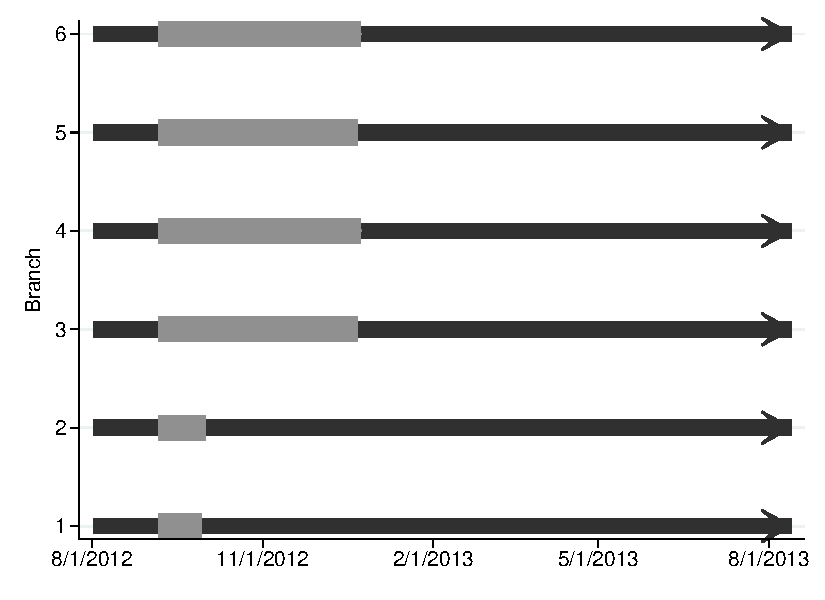
\includegraphics[width=\textwidth]{Figuras/timeline_suc_exp_extended.pdf}
    \end{subfigure}
    \begin{subfigure}{0.45\textwidth}
    \caption{Experiment arms}
       \centering
      \includegraphics[width=\textwidth]{Figuras/exp_arms.PNG}
    \end{subfigure}
    \end{center}
         \scriptsize Panel (a) displays in black arrows the period covered by our administrative data: from \hl{XXX} (\hl{XXX} days before the experiment began) to \hl{XXX}. The gray lines arrows correspond to the dates of implementation of the experiment. We finished the experiment earlier in branches 1 and 2 because we realized that we would have enough sample size with the remaining branches and save on operational costs. Panel (b) shows our 5 treatment arms: control (status quo contract), no choice with fee, no choice with promise, choice among both contracts where the commitment contract has a fee, and choice among both contracts where the commitment contract involves only a promise. Within each arm it displays the number of observations. And  for the choice groups it splits the sample size into those who chose the commitment contract (shaded blue triangle) and those that did not (un-shaded triangle).
      \textit{Do file: }  \texttt{timeline\_suc\_exp.do}
\end{figure}



\begin{figure}[H]
     \caption{Explanatory Material: Promise-Choice Days}
    \label{ExplanatoryMaterial}
    \begin{center}
    \begin{subfigure}{0.8\textwidth}
        \centering
        \includegraphics[width=\textwidth]{Figuras/MicaChoiceDonde.png}
    \end{subfigure}
    \end{center}
    \scriptsize
        xxx
\end{figure}





\begin{figure}[H]
     \caption{Financial cost}
    \label{fc_hist}
    \begin{center}
    \begin{subfigure}{.45\textwidth}
      \caption{In pesos}
        \centering
        \includegraphics[width=\textwidth]{Figuras/hist_fc.pdf}
    \end{subfigure}
    \begin{subfigure}{0.45\textwidth}
    \caption{As a fraction of the loan}
       \centering
      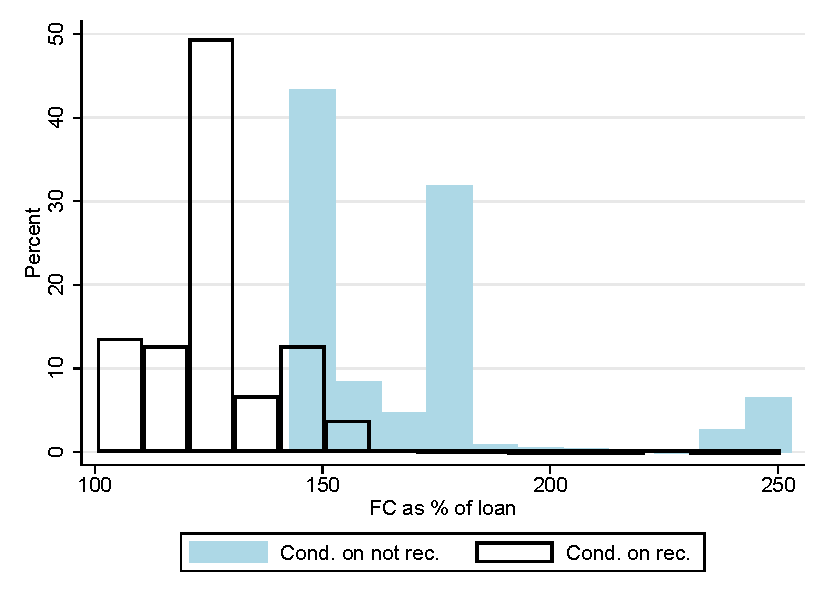
\includegraphics[width=\textwidth]{Figuras/hist_fc_perc_loan.pdf}
    \end{subfigure}
    \end{center}
         \scriptsize
         Panel (a) presents a histogram of financial cost for the control group. Financial cost is defined as the sum of payments made by a client towards recovering her pawn + the cost of the pawned piece when she ends up losing it. In the paper we use different costs of losing the pawn: its value in gold, or the self reported subjective (e.g. jewelry may have sentimental value). This Figure uses the \hlgr{gold value}. We plot separately the financial cost for those who lose the pawn (blue) and those that recover it (transparent).  Panel (b) is analogous but we normalized the financial cost dividing it by the loan size.  %Given that the loan lasts close to 90 days, bringing payments to present value makes little difference. 
      %\footnotesize{ } \textit{Do file: }  \texttt{hist\_fc.do}
\end{figure}






\begin{figure}[H]
    \caption{The effect of the fee-forcing treatment}
    \label{fc_pro2}
    \begin{center}
    \begin{subfigure}{0.45\textwidth}
        \caption{Financial cost}
        \centering
        \includegraphics[width=\textwidth]{Figuras/fc_te_pro_2.pdf}
    \end{subfigure}
        \begin{subfigure}{0.45\textwidth}
        \caption{Financial cost (quantile reg)}
        \centering
        \includegraphics[width=\textwidth]{Figuras/fc_quantile_pro_2.pdf}
    \end{subfigure}
    
        \bigskip
        \bigskip
    
    \begin{subfigure}{0.45\textwidth}
        \caption{Financial cost (HTE)}
        \centering
        \includegraphics[width=\textwidth]{Figuras/he_dist_fc_admin_disc_pro_2.pdf}
    \end{subfigure}
    \begin{subfigure}{0.45\textwidth}
        \caption{Lost pawn}
        \centering
        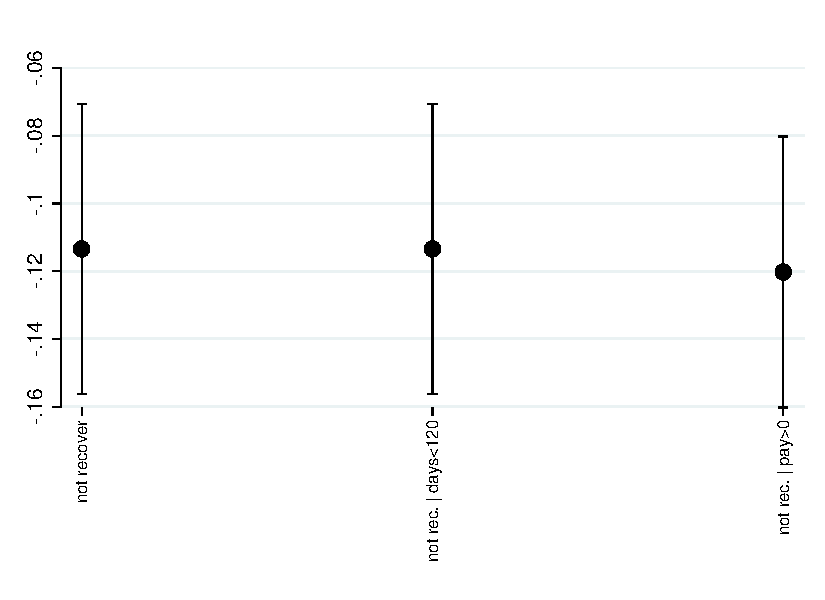
\includegraphics[width=\textwidth]{Figuras/def_te_pro_2.pdf}
    \end{subfigure}

    \end{center}
        \scriptsize 
        This figure shows the estimated treatment effect of ``forcing'' the frequent payment commitment contract using fees, compared to the status-quo (control) for  financial cost (Panel a), quantiles of financial cost (Panel b), and for an indicator of losing the pawn (Panel c). In Panel (a) each dot represents the estimated treatment effect for a different definition of financing cost, or for a different sub-population, and its 95\% confidence interval. From left to right, the first effect corresponds to using the gold value of the pawned piece in the definition of financial cost and discounting the payments to present value using a \hl{XXX} monthly rate; the second uses the subjective value of the pawn; the third is analogous to the second but adds transaction cost (transport+1 day's wage) per visit; the fourth conditions on the population that paid any positive amount towards recovery of their pawn; the fifth conditions on the sub-population \hl{of the treatment group} that paid a fee and \hl{compares these to all the control group}; the sixth conditions on the intersection of the previous two sub-populations. Panel (b) plots the effects on different quantiles of the distribution of financial cost (\hl{using the first definition}): 15th, 25th, 50th, 75th, 85th percentile. Panel (c) Measures the effect of treatment on the likelihood of losing their pawn. The first coefficient compares all the treatment group vs all the control; the second conditions on the population that paid any positive amount towards recovery of their pawn; the third conditions on having paid at least 30\% of the loan amount; the fourth conditions on the period covering the first cycle of the loan; the fifth on the period of the first cycle and paying any positive amount. The distribution plots the FC treatment effect for the interval $[\mu-2\sigma,\mu+2\sigma]$ to ignore the outliers. Panel (d) plots the distribution of the heterogeneous treatment effects on financial cost, estimated using \hl{Athey Wagner XXX}. % the effect on ``repeat purchase''. That is likelihood of doing an additional pawn (in treatment vs control) after having been subjected to treatment for at least 75 days. The second coefficient estimates the regression conditional on recovering the pawn \hl{in both treatment and control}, and the rightmost coefficient compares those above the median treatment effect in financial cost savings, \hl{versus all the control group.}
      %\textit{Do file: }  \texttt{fc\_te.do, def\_te.do, fc\_quantilereg.do}
\end{figure}





\begin{figure}[H]
        \caption{Effects on repeat purchasing}
    \label{reincidence}
    \begin{center}
        \centering
        \includegraphics[width=0.6\textwidth]{re_te.pdf}
    \end{center}
     \footnotesize \textit{Notes: } 
      \footnotesize{ \textit{Do file: }  \texttt{re\_te.do}}
\end{figure}




\begin{figure}[H]
    \caption{The effect choice between fee-commitment and status quo}
    \label{fc_pro4}
    \begin{center}
    \begin{subfigure}{0.45\textwidth}
        \caption{Financial cost}
        \centering
        \includegraphics[width=\textwidth]{Figuras/fc_te_pro_4.pdf}
    \end{subfigure}
        \begin{subfigure}{0.45\textwidth}
        \caption{Financial Cost (quantile reg)}
        \centering
        \includegraphics[width=\textwidth]{Figuras/fc_quantile_pro_4.pdf}
    \end{subfigure}
    \begin{subfigure}{0.5\textwidth}
    
        \bigskip
        \bigskip
    
        \caption{Lost Pawn}
        \centering
        \includegraphics[width=\textwidth]{Figuras/def_te_pro_4.pdf}
    \end{subfigure}
    \end{center}
        \scriptsize
        This figure is analogous to Figure \ref{fc_pro2}. It measures the effect of being given \textit{choice} between the frequent payment commitment contract and the status-quo contract versus being \textit{``forced''} into the status-quo contract (control). Again it focuses our two main outcomes: financial cost and an indicator for losing the pawn. However, it also presents differences in these two outcomes for those who chose the frequent payment commitment contract versus the whole control group (squares-NSQ), and also for those who chose the status quo contract versus the whole control group (triangles-SQ). Note that these two comparisons are not pure causal effects since people who chose the frequent payment commitment contract may be different from those that do not. That is: the squares and triangles combine selection and treatment effects. Finally, for comparison purposes, the blue diamonds display the effects of forcing them into the frequent payment commitment contract and are just transcribed from Figure \ref{fc_pro2} above. 
      \textit{Do file: }  \texttt{fc\_te\_choice\_dec.do, def\_te\_choice\_dec.do, fc\_quantilereg\_choice\_dec.do}
\end{figure}



\begin{figure}[H]
    \caption{Choice of contracts and treatment effects}
    \label{choose_wrong}
    \begin{center}
        \begin{subfigure}{0.45\textwidth}
        \caption{Chose wrong}
        \centering
        \includegraphics[width=\textwidth]{Figuras/line_cw_fc_te_cf.pdf}
        
    \end{subfigure}
        \begin{subfigure}{0.45\textwidth}
        \caption{By overconfidence/naivete}
        \centering
        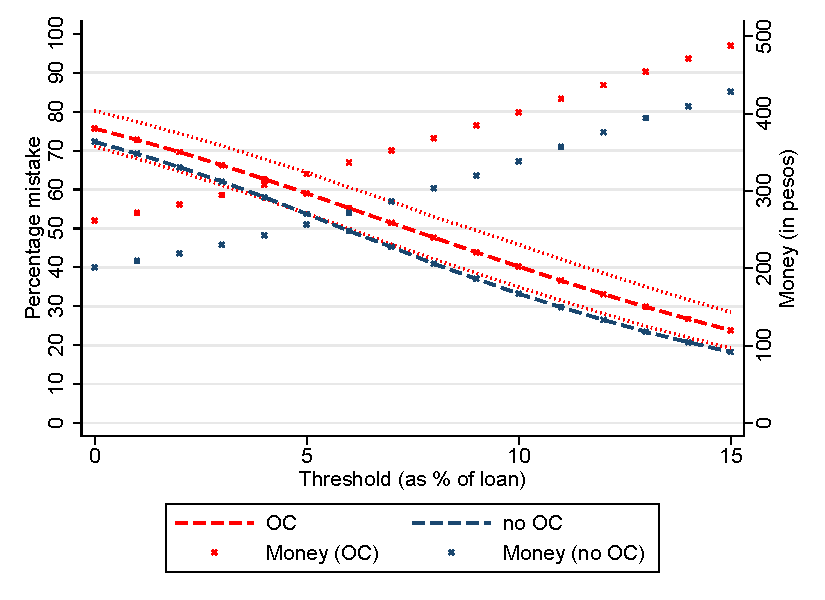
\includegraphics[width=\textwidth]{Figuras/line_cw_fc_te_cf_OC_fee.pdf}

    \bigskip
        
    \end{subfigure}
        \begin{subfigure}{0.45\textwidth}
        \caption{\% better when forced to fee-commitment}
        \centering
        \includegraphics[width=\textwidth]{Figuras/line_better_forceall_fc_te_cf.pdf}
        
    \end{subfigure}
        \begin{subfigure}{0.45\textwidth}
        \caption{\footnotesize{Effect of losing pawn vs predicted take-up}}
        \centering
        \includegraphics[width=\textwidth]{Figuras/takeuppr_def.pdf}
    \end{subfigure}
    
    \end{center}
        \scriptsize
        \hl{Es correcto esto que escribi isaac?} Panel (a) aims to show that subjects with higher  treatment effect in the no-choice arm (using \hl{Athey and Wagner (XXX) heterogeneous treatment effect estimator ISAAC puedes meter aqui el cite?}) are \textit{not} more likely to chose it if given choice. We proceed in three steps: first, within the choice arm, we estimate the probability of taking up the commitment contract ($\widehat{P(x_i)}$) using random forests, the baseline survey and pre-treatment administrative data. Second, we extrapolate these predictions to the no-choice and control arms using the $x_i$'s. Finally, We allocate subjects into 5 groups according to whether their predicted probability $\widehat{P(x_i)}$ is in \hl{[0,10],(10,20],(50,70],(30,}, and for each of these sub-populations separately we estimate the ATE of the no-choice treatment using regression equation \hl{XXX}. We find that take up of treatment is \textit{not} correlated with the benefit of treatment, if anything the correlation is negative. Panel (b) does almost the reverse procedure. We estimate what the treatment effect of the commitment contract \textit{would have been} for all subjects in the choice arm if they had been forced into it. To do this we estimate heterogeneous treatment effects as a function of our $x$'s in the no-choice arm, and extrapolate them to the choice arm. With these in hand, we calculate what fraction of subjects in the choice arm incurred in \hl{financial costs that are  $\geq Z$\% than if they had chosen the opposite contract of what they actually chose.} We define $Z$\% as a fraction of the loan in the X-axis. The left Y-axis measures the fraction of subjects, and \hl{the right Y-axis measures the amount of money ``left on the table''.} 
        \textit{Do file: }  \texttt{effect\_contr\_takeup.do, choose\_wrong\_quant\_wrong.do, choose\_wrong\_quant\_wrong\_decomposition.do}
\end{figure}






\begin{figure}[H]
    \caption{The effect of choice between promise-commitment and status quo}
    \label{fc_pro5}
    \begin{center}
    \begin{subfigure}{0.45\textwidth}
        \caption{Financial cost -- Choice}
        \centering
        \includegraphics[width=\textwidth]{Figuras/fc_te_pro_5.pdf}
    \end{subfigure}
        %\begin{subfigure}{0.45\textwidth}
        %\caption{Quantile regression}
        %\centering
        %\includegraphics[width=\textwidth]{Figuras/fc_quantile_pro_5.pdf}
    %\end{subfigure}
    \begin{subfigure}{0.45\textwidth}
        \caption{Losing Pawn -- Choice}
        \centering
        \includegraphics[width=\textwidth]{Figuras/def_te_pro_5.pdf}
    \end{subfigure}
    
    \bigskip
    \bigskip
    
    \begin{subfigure}{0.45\textwidth}
        \caption{Financial cost -- Promise-forcing}
        \centering
        \includegraphics[width=\textwidth]{Figuras/fc_te_pro_3.pdf}
    \end{subfigure}
    \begin{subfigure}{0.45\textwidth}
        \caption{Losing Pawn -- Promise-forcing}
        \centering
        \includegraphics[width=\textwidth]{Figuras/def_te_pro_3.pdf}
    \end{subfigure}
    \end{center}
             \footnotesize \textit{Notes: } 
      \footnotesize{ } \textit{Do file: }  \texttt{fc\_te\_choice\_dec.do, def\_te\_choice\_dec.do, fc\_quantilereg\_choice\_dec.do}
\end{figure}




%\begin{figure}[H]
%    \caption{The effect of the promise-forcing treatment}
%    \label{fc_pro3}
%    \begin{center}
%        \begin{subfigure}{0.45\textwidth}
%        \caption{Quantile regression}
%        \centering
%        \includegraphics[width=\textwidth]{Figuras/fc_quantile_pro_3.pdf}
%    \end{subfigure}
%    
%    \end{center}
%             \footnotesize \textit{Notes: } 
%      \footnotesize{ } \textit{Do file: }  \texttt{fc\_te.do, def\_te.do, fc\_quantilereg.do}
%\end{figure}








\pagebreak


%%%%%%%%%%%%%%%%%%%%%%%%%%%%%%%%%%%%%%%%%%%%%%%

% APPENDIX TABLES


\setcounter{table}{0}
\renewcommand{\thetable}{A\arabic{table}}

\setcounter{figure}{0}
\renewcommand{\thefigure}{A\arabic{figure}}

\setcounter{section}{0}
\setcounter{subsection}{0}
\renewcommand\thesection{A\arabic{section}}
\renewcommand\thesubsection{\thesection\arabic{subsection}}

\appendix

\section{APPENDIX}

\subsection{Tables}


\begin{table}[H]
\caption{Balance response table}
\label{balance_response}
\begin{center}
\scriptsize{% Table generated by Excel2LaTeX from sheet 'balance_response'
\begin{tabular}{lcccc|ccc}
\toprule
      &       & \multicolumn{3}{c|}{Panel A : Baseline Survey} & \multicolumn{3}{c}{Panel B : Exit Survey} \\
\midrule
\midrule
      & Overall & No Response & Response & p-value & No Response & Response & p-value \\
\midrule
\midrule
Loan amount  & 2153.78 & 2194.85 & 2153.78 & 0.53  & 2157.15 & 2367.62 & 0.17 \\
      & (31.82) & (50.16) & (41.81) &       & (30.93) & (154.83) &  \\
Monday & 0.18  & 0.19  & 0.18  & 0.66  & 0.18  & 0.19  & 0.71 \\
      & (0.02) & (0.02) & (0.03) &       & (0.02) & (0.04) &  \\
Pawns & 46.22 & 43.19 & 48.48 & 0     & 46.41 & 43.58 & 0.08 \\
      & (2.08) & (1.8) & (2.36) &       & (2.1) & (2.34) &  \\
\midrule
Obs   & 13444 & 5740  & 7704  &       & 12539 & 905   &  \\
\bottomrule
\bottomrule
\end{tabular}%
}
\end{center}
 \scriptsize
%\textit{Do file: } \texttt{balance\_response.do}
\end{table}



\begin{table}[H]
    \caption{Out of sample measures of fit}
    \label{Table_compliance}
    \begin{subtable}{1\textwidth}
      \centering
        \caption{Take up}
        \scriptsize{% Table generated by Excel2LaTeX from sheet 'oos_pago_frec_vol'
\begin{tabular}{lcccc}
\toprule
      & \multicolumn{4}{c}{Choice} \\
\midrule
\midrule
GOF measures & Logit & SW-Logit & RF    & Boosting \\
\midrule
\midrule
AUC (out of sample) & 0.77  & 0.76  & 0.8   & 0.77 \\
      & (0.04) & (0.04) & (0.04) & (0.04) \\
AUC (in sample) & 0.76  & 0.75  & 0.87  & 0.84 \\
      & (0.02) & (0.02) & (0.01) & (0.01) \\
Accuracy & 0.77  & 0.78  & 0.75  & 0.78 \\
\bottomrule
\bottomrule
\end{tabular}%
}
    \end{subtable}%
    
    \bigskip
    \begin{subtable}{1\textwidth}
      \centering
        \caption{Take up w/Fee}
        \scriptsize{% Table generated by Excel2LaTeX from sheet 'oos_pago_frec_vol_fee'
\begin{tabular}{lcccc}
\toprule
      & \multicolumn{4}{c}{Frequent voluntary payment - FEE} \\
\midrule
\midrule
OOS measures & Logit & SW-Logit & RF    & Boosting \\
\midrule
\midrule
MAE   & 0.21  & 0.21  & 0.23  & 0.17 \\
MSE   & 0.1   & 0.1   & 0.1   & 0.09 \\
AUC (out of sample) & 0.76  & 0.78  & 0.84  & 0.85 \\
      & (0.06) & (0.06) & (0.06) & (0.05) \\
AUC (in sample) & 0.84  & 0.82  & 0.92  & 0.99 \\
      & (0.02) & (0.02) & (0.01) & (0.01) \\
Accuracy & 0.82  & 0.84  & 0.86  & 0.88 \\
Correlation (0-1) & 0.13  & 0.26  & 0.37  & 0.31 \\
Correlation (predicted val) & 0.33  & 0.38  & 0.37  & 0.43 \\
R-squared  & 0.08  & 0.13  & 0.11  & 0.19 \\
Expected value of predictions & 0.17  & 0.17  & 0.16  & 0.12 \\
\bottomrule
\bottomrule
\end{tabular}%
}
    \end{subtable}
    
      \bigskip
    \begin{subtable}{1\textwidth}
      \centering
        \caption{Take up w/promise}
        \scriptsize{% Table generated by Excel2LaTeX from sheet 'oos_pago_frec_vol_promise'
\begin{tabular}{lcccc}
\toprule
      & \multicolumn{4}{c}{Choice-Promise Arm} \\
\midrule
\midrule
GOF measures & Logit & SW-Logit & RF    & Boosting \\
\midrule
\midrule
AUC (out of sample) & 0.63  & 0.63  & 0.7   & 0.72 \\
      & (0.06) & (0.06) & (0.06) & (0.06) \\
AUC (in sample) & 0.83  & 0.82  & 0.9   & 0.97 \\
      & (0.02) & (0.02) & (0.01) & (0.01) \\
Accuracy & 0.62  & 0.67  & 0.65  & 0.7 \\
\bottomrule
\bottomrule
\end{tabular}%
}
    \end{subtable}
            \scriptsize
           \\
           \\
           \\
  \textit{Notes:} 
    
     \textit{Scripts: } \texttt{pred\_take\_up.do, pfv\_pred.R}
\end{table}




\begin{table}[H]
\caption{Reincidence SS}
\label{tab_reincidence}
\begin{center}
\scriptsize{% Table generated by Excel2LaTeX from sheet 'tab_reincidence'
\begin{tabular}{lccccc}
\toprule
Variable & Obs   & Mean  & Std. Dev. & Min   & Max \\
\midrule
\midrule
Number of visits & 26179 & 1.72  & 1.27  & 1     & 7 \\
Received more one treatment arm & 26179 & 0.23  & 0.42  & 0     & 1 \\
Number of arms & 26179 & 1     & 1.06  & 0     & 5 \\
Reincidence & 16470 & 0.29  & 0.45  & 0     & 1 \\
Same product of reincidence & 16470 & 0.02  & 0.13  & 0     & 1 \\
Number of visits $<$ 75 days & 26179 & 2.1   & 1.5   & 1     & 7 \\
Received more one treatment arm $<$ 75 days & 26179 & 0.22  & 0.41  & 0     & 1 \\
Number of arms  $<$ 75 days & 26179 & 0.97  & 1.01  & 0     & 5 \\
Chose same treatment arm & 1066  & 0.45  & 0.5   & 0     & 1 \\
\bottomrule
\bottomrule
\end{tabular}%
}
\end{center}
 \scriptsize
%\textit{Do file: } \texttt{tab\_reincidence.do}
\end{table}




\begin{table}[H]
\caption{Summary statistics (exit survey)}
\label{SS_exit}
\begin{center}
\scriptsize{% Table generated by Excel2LaTeX from sheet 'SS'
\begin{tabular}{lccccccc}
\toprule
\multicolumn{8}{c}{Exit Survey Data} \\
\midrule
\midrule
      &       &       & \multicolumn{2}{c}{No Choice } & \multicolumn{2}{c}{Choice} &  \\
\midrule
\midrule
      & Overall & Control & Fee   & Promise & Fee   & Promise & p-value \\
\midrule
      & \multicolumn{7}{c}{Panel A: Outcomes} \\
\midrule
\midrule
Will reincide & 0.94  & 0.96  & 0.95  & 0.96  & 0.94  & 0.92  & 0.6 \\
      & (0.01) & (0.01) & (0.02) & (0.02) & (0.02) & (0.03) &  \\
Very satisfied & 0.34  & 0.36  & 0.32  & 0.33  & 0.33  & 0.36  & 0.95 \\
      & (0.02) & (0.05) & (0.05) & (0.05) & (0.04) & (0.04) &  \\
Better econ situation & 0.42  & 0.53  & 0.29*** & 0.35** & 0.44  & 0.47  & 0.02 \\
      & (0.03) & (0.06) & (0.05) & (0.06) & (0.05) & (0.04) &  \\
Choose frequent payment & 0.63  & 0.65  & 0.58  & 0.58  & 0.58  & 0.77** & 0 \\
      & (0.02) & (0.05) & (0.05) & (0.06) & (0.04) & (0.03) &  \\
\midrule
      & \multicolumn{7}{c}{Panel B: Balance} \\
\midrule
\midrule
Loan amount  & 1957.72 & 1940.41 & 1926  & 2006.83 & 2002.97 & 1892.54 & 0.98 \\
      & (67.84) & (160.03) & (150.89) & (187.56) & (114.96) & (157.83) &  \\
Woman & 0.71  & 0.69  & 0.72  & 0.77  & 0.66  & 0.73  & 0.58 \\
      & (0.02) & (0.05) & (0.06) & (0.05) & (0.05) & (0.04) &  \\
Age   & 43.98 & 42.84 & 46.27 & 43.82 & 44.57 & 42.24 & 0.29 \\
      & (0.59) & (1.33) & (1.74) & (1.1) & (0.99) & (1.16) &  \\
Subjective value & 3166.31 & 3448.99 & 3182.11 & 3049.88 & 3074.69 & 3081.52 & 0.85 \\
      & (120.82) & (288.38) & (286.2) & (303.87) & (210.79) & (296.63) &  \\
Has pawn before & 0.88  & 0.84  & 0.9   & 0.87  & 0.95** & 0.8   & 0.01 \\
      & (0.02) & (0.05) & (0.03) & (0.05) & (0.02) & (0.05) &  \\
Subj. pr. of recovery & 95.35 & 94.5  & 94.84 & 96.6  & 95.06 & 95.87 & 0.82 \\
      & (0.56) & (1.4) & (1.21) & (1.5) & (1.01) & (1.09) &  \\
+High-school & 0.66  & 0.72  & 0.63  & 0.65  & 0.67  & 0.64  & 0.84 \\
      & (0.03) & (0.06) & (0.06) & (0.07) & (0.05) & (0.06) &  \\
\midrule
Obs   & 905   & 175   & 154   & 172   & 234   & 170   &  \\
\bottomrule
\bottomrule
\end{tabular}%
}
\end{center}
 \footnotesize
\textit{Notes:} 

\textit{Do file: } \texttt{ss.do}
\end{table}



\begin{table}[H]
\caption{Stochastic dominance of fee-forcing contract}
\label{stochastic_dominance}
\begin{center}
\scriptsize{% Table generated by Excel2LaTeX from sheet 'dominance'
\begin{tabular}{lccc}
\toprule
Sub-population & Dominance & Log-normality (AD/KS) & Obs \\
\midrule
\midrule
Fee-forcing & \cellcolor[rgb]{ .557,  .663,  .859} $\succeq_{1}^*$ & */*  |  */* & 5034 \\
Low-loan & $\succeq_{1}^*$ &    /     |     /    & 2508 \\
High-loan & $\succeq_{1}^*$ &    /     |     /    & 2526 \\
Low-subj. prob. & \cellcolor[rgb]{ .557,  .663,  .859} $\succeq_{1}^*$ & */*  |  */* & 1083 \\
High-subj. Prob. & \cellcolor[rgb]{ .557,  .663,  .859} $\succeq_{1}^*$ & */*  |  */* & 2590 \\
Low-age & $\preceq_{1}$ & */*  |  */* & 1358 \\
High-age & \cellcolor[rgb]{ .851,  .882,  .949} $\succeq_{1}$ & */*  |     /* & 1363 \\
Low-income index & \cellcolor[rgb]{ .851,  .882,  .949} $\succeq_{1}$ & */*  |  */* & 1047 \\
High-income index & \cellcolor[rgb]{ .851,  .882,  .949} $\succeq_{1}$ & */*  |  */* & 948 \\
Male  & -     & */*  |     /* & 756 \\
Female & \cellcolor[rgb]{ .851,  .882,  .949} $\succeq_{1}$ & */*  |  */* & 2158 \\
First time & $\preceq_{1}$ & */*  |  */* & 293 \\
Pawn before & \cellcolor[rgb]{ .851,  .882,  .949} $\succeq_{1}$ & */*  |  */* & 2476 \\
Family doesn't ask & $\preceq_{1}$ & */*  |  */* & 1826 \\
Family asks & \cellcolor[rgb]{ .557,  .663,  .859} $\succeq_{1}^*$ & */*  |  */* & 988 \\
Not common ask & \cellcolor[rgb]{ .851,  .882,  .949} $\succeq_{1}$ & */*  |  */* & 1436 \\
Common asks & -     & */*  |  */* & 625 \\
No savings & $\preceq_{1}$ & */*  |  */* & 1353 \\
Has savings & \cellcolor[rgb]{ .557,  .663,  .859} $\succeq_{1}^*$ & */*  |  */* & 717 \\
Not rosca & \cellcolor[rgb]{ .557,  .663,  .859} $\succeq_{1}^*$ & */*  |  */* & 1270 \\
Rosca & $\preceq_{1}$ & */*  |  */* & 795 \\
Low-education & \cellcolor[rgb]{ .851,  .882,  .949} $\succeq_{1}$ & */*  |     /* & 906 \\
High-education & \cellcolor[rgb]{ .851,  .882,  .949} $\succeq_{1}$ & */*  |  */* & 1798 \\
Not stressed & -     & */*  |  */* & 1999 \\
Stressed & -     & */*  |  */* & 839 \\
Not overconfident & \cellcolor[rgb]{ .557,  .663,  .859} $\succeq_{1}^*$ & */*  |  */* & 68 \\
Overconfident & \cellcolor[rgb]{ .851,  .882,  .949} $\succeq_{1}$ & */*  |     /* & 1605 \\
Not PB & \cellcolor[rgb]{ .851,  .882,  .949} $\succeq_{1}$ & */*  |  */* & 1438 \\
PB    & \cellcolor[rgb]{ .557,  .663,  .859} $\succeq_{1}^*$ & */*  |     /* & 226 \\
Not FB & \cellcolor[rgb]{ .851,  .882,  .949} $\succeq_{1}$ & */*  |  */* & 1521 \\
FB    & \cellcolor[rgb]{ .851,  .882,  .949} $\succeq_{1}$ & */*  |  */* & 143 \\
Doesn't make budget & \cellcolor[rgb]{ .851,  .882,  .949} $\succeq_{1}$ & */*  |  */* & 1055 \\
Makes budget & \cellcolor[rgb]{ .851,  .882,  .949} $\succeq_{1}$ & */*  |  */* & 1689 \\
Not tempted & \cellcolor[rgb]{ .851,  .882,  .949} $\succeq_{1}$ & */*  |     /* & 875 \\
Tempted & \cellcolor[rgb]{ .851,  .882,  .949} $\succeq_{1}$ & */*  |  */* & 1873 \\
High-transp. cost & \cellcolor[rgb]{ .851,  .882,  .949} $\succeq_{1}$ & */*  |  */* & 1353 \\
Low-transp. cost & \cellcolor[rgb]{ .851,  .882,  .949} $\succeq_{1}$ & */*  |  */* & 1343 \\
High-transp. time & \cellcolor[rgb]{ .851,  .882,  .949} $\succeq_{1}$ & */*  |  */* & 1260 \\
Low-transp. time & \cellcolor[rgb]{ .557,  .663,  .859} $\succeq_{1}^*$ & */*  |  */* & 1443 \\
\bottomrule
\bottomrule
\end{tabular}%
}
\end{center}
 \footnotesize
\textit{Notes:} 

\textit{Do file: } \texttt{stoch\_dominance.do}
\end{table}

\begin{table}[H]
\caption{OC Regression}
\label{oc_reg}
\begin{center}
\scriptsize{% Table generated by Excel2LaTeX from sheet 'oc_reg'
\begin{tabular}{lcccccc}
\toprule
      & \multicolumn{4}{c}{Take-up (choice arms)} & \multicolumn{2}{c}{Financing Cost (hte)} \\
\midrule
\midrule
      & Fee   & Fee   & Promise & Promise &       &  \\
\midrule
      & (1)   & (2)   & (3)   & (4)   & (5)   & (6) \\
\midrule
\midrule
OC (dummy) & -0.13 & -0.16 & 0.021 & -0.012 & -133.2 & -129.7 \\
      & (0.070) & (0.084) & (0.097) & (0.14) & (37.1) & (38.7) \\
Constant  & 0.24  & 0.18  & 0.62  & 0.50  & -324.3 & -306.9 \\
      & (0.084) & (0.11) & (0.12) & (0.17) & (67.6) & (68.5) \\
      &       &       &       &       &       &  \\
\midrule
Observations & 1024  & 778   & 838   & 677   & 1259  & 1259 \\
R-sq  & 0.139 & 0.162 & 0.189 & 0.223 & 0.042 & 0.044 \\
Dep. Var. Mean & 0.14  & 0.15  & 0.36  & 0.36  & \multicolumn{2}{c}{-327.4} \\
Branch/Day FE & \checkmark & \checkmark & \checkmark & \checkmark & \checkmark & \checkmark \\
Controls &       & \checkmark &       & \checkmark &       & \checkmark \\
\bottomrule
\bottomrule
\end{tabular}%
}
\end{center}
 \footnotesize
\textit{Notes:} 

\textit{Do file: } \texttt{oc.do}
\end{table}


\pagebreak



\subsection{Figures}


\begin{figure}[H]
     \caption{Contract Terms Summary, and Promise Slip}
    \label{PaperSlip}
    \begin{center}
    \begin{subfigure}{0.75\textwidth}
        \centering
        \includegraphics[width=\textwidth]{Figuras/ContractDonde.png}
    \end{subfigure}
    \begin{subfigure}{0.4\textwidth}
        \centering
        \includegraphics[width=\textwidth]{Figuras/PersonalPromise.png}
    \end{subfigure}
    \end{center}
    \scriptsize
         xxx 
\end{figure}

\begin{figure}[H]
        \caption{ECDF of Financial Cost}
    \label{ecdf_fc}
    \begin{center}
        \centering
        \includegraphics[width=0.5\textwidth]{Figuras/cdf_fc_pro_2.pdf}
    \end{center}
    \footnotesize \textit{Notes: } 
     \footnotesize{ \textit{Do file: }  \texttt{hist\_fc.do}}
\end{figure}


\begin{figure}[H]
    \caption{Behavior of those who lost pawn}
    \label{proxy_naive}
    \begin{center}
    \begin{subfigure}{0.40\textwidth}
        \caption{Elapsed days to first payment}
        \centering
        \includegraphics[width=\textwidth]{Figuras/hist_firstdays_default.pdf}
    \end{subfigure}
    \begin{subfigure}{0.40\textwidth}
        \caption{Elapsed days to last payment}
        \centering
        \includegraphics[width=\textwidth]{Figuras/hist_days_default.pdf}
    \end{subfigure}
        \begin{subfigure}{0.40\textwidth}
        \caption{Payments as \% of loan}
        \centering
        \includegraphics[width=\textwidth]{Figuras/hist_percpay_default.pdf}
    \end{subfigure}
    \begin{subfigure}{0.40\textwidth}
        \caption{Number of payments}
        \centering
        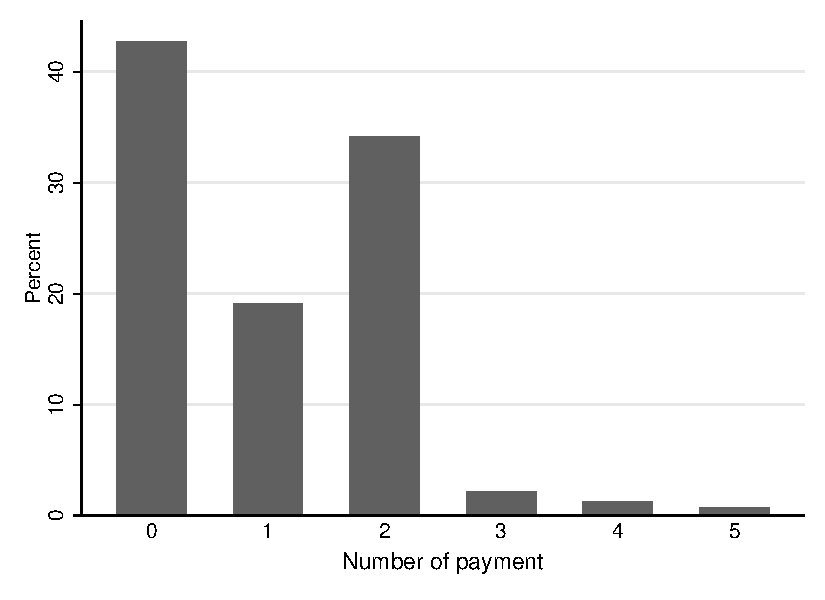
\includegraphics[width=\textwidth]{Figuras/hist_numpay_default.pdf}
    \end{subfigure}
    \end{center}
        \scriptsize 
        This figure describes behavior for the subsample of clients whose pawn was not recovered (\hl{in the control group}).  Panel (a) shows days elapsed from the pawn to the first payment, while panel (b) displays the days elapsed to last payment. Some people pay after the day 105 when the grace period ends because the can ``restart'' the loan if they pay all interest owed. It amounts to starting a new loan \hl{with the same conditions} and same pawn. Panel (c) shows the fraction of the loan that they paid (even when they ended up losing the pawn). Panel (d) displays the number of times they went to the branch to pay.      
      \textit{Do file: }  \texttt{hist\_den\_default.do}
\end{figure}



%\begin{figure}[H]
%        \caption{Booklet with product information}
%    \label{micas}
%    \begin{center}
%        \centering
%        \includegraphics[width=\textwidth]{micas.pdf}
%    \end{center}
%     \footnotesize \textit{Notes: } 
%      \footnotesize{ }
%\end{figure}


%\begin{figure}[H]
%     \caption{Booklet with product information translated}
%    \label{booklet_translate2}
%    \begin{center}
%    \begin{subfigure}{.9\textwidth}
%        \centering
%        \includegraphics[width=\textwidth]{Figuras/MP_F.pdf}
%    \end{subfigure}
    %\begin{subfigure}{0.55\textwidth}
    %   \centering
    %  \includegraphics[width=\textwidth]{Figuras/MP_2.pdf}
    %\end{subfigure}
%    \end{center}
%\end{figure}



\begin{figure}[H]
        \caption{Histogram of payments}
    \label{HistPayments}
    \begin{center}
    \begin{subfigure}{.31\textwidth}
    \caption{Control}
        \centering
        \includegraphics[width=\textwidth]{Figuras/hist_payments_pro_1.pdf}
    \end{subfigure}
    \begin{subfigure}{.31\textwidth}
    \caption{Forcing - fee}
        \centering
        \includegraphics[width=\textwidth]{Figuras/hist_payments_pro_2.pdf}
    \end{subfigure}   
     \begin{subfigure}{.31\textwidth}
    \caption{Forcing - promise}
        \centering
        \includegraphics[width=\textwidth]{Figuras/hist_payments_pro_3.pdf}
    \end{subfigure}  
     \begin{subfigure}{.31\textwidth}
    \caption{Choice - fee}
        \centering
        \includegraphics[width=\textwidth]{Figuras/hist_payments_pro_4.pdf}
    \end{subfigure}  
     \begin{subfigure}{.31\textwidth}
    \caption{Choice - fee - SQ}
        \centering
        \includegraphics[width=\textwidth]{Figuras/hist_payments_pro_6.pdf}
    \end{subfigure}    
     \begin{subfigure}{.31\textwidth}
    \caption{Choice - fee - NSQ}
        \centering
        \includegraphics[width=\textwidth]{Figuras/hist_payments_pro_7.pdf}
    \end{subfigure}    
     \begin{subfigure}{.31\textwidth}
    \caption{Choice - promise}
        \centering
        \includegraphics[width=\textwidth]{Figuras/hist_payments_pro_5.pdf}
    \end{subfigure}  
     \begin{subfigure}{.31\textwidth}
    \caption{Choice - promise - SQ}
        \centering
        \includegraphics[width=\textwidth]{Figuras/hist_payments_pro_8.pdf}
    \end{subfigure}    
     \begin{subfigure}{.31\textwidth}
    \caption{Choice - promise - NSQ}
        \centering
        \includegraphics[width=\textwidth]{Figuras/hist_payments_pro_9.pdf}    
    \end{subfigure}        
    \end{center}
     \footnotesize \textit{Notes: } The x-axis shows the elapsed days between initial date and current movement.
      \footnotesize{ \textit{Do file: }  \texttt{hist\_payments.do}}
\end{figure}

%\begin{figure}[H]
%        \caption{Types of agents that incur in different FC}
%    \label{components_fc}
%    \begin{center}
%        \centering
%        \includegraphics[width=\textwidth]{Figuras/scatter_fc_pay.pdf}
%    \end{center}
%     \footnotesize \textit{Notes: } 
%      \footnotesize{ \textit{Do file: }  \texttt{hist\_fc.do}}
%\end{figure}




\begin{figure}[H]
        \caption{Percentage of payments}
    \label{perc_payments}
    \begin{center}
    \begin{subfigure}{.31\textwidth}
    \caption{Control}
        \centering
        \includegraphics[width=\textwidth]{Figuras/hist_porc_pay_pro_1.pdf}
    \end{subfigure}
    \begin{subfigure}{.31\textwidth}
    \caption{Forcing - fee}
        \centering
        \includegraphics[width=\textwidth]{Figuras/hist_porc_pay_pro_2.pdf}
    \end{subfigure}   
     \begin{subfigure}{.31\textwidth}
    \caption{Forcing - promise}
        \centering
        \includegraphics[width=\textwidth]{Figuras/hist_porc_pay_pro_3.pdf}
    \end{subfigure}  
     \begin{subfigure}{.31\textwidth}
    \caption{Choice - fee}
        \centering
        \includegraphics[width=\textwidth]{Figuras/hist_porc_pay_pro_4.pdf}
    \end{subfigure}  
     \begin{subfigure}{.31\textwidth}
    \caption{Choice - fee - SQ}
        \centering
        \includegraphics[width=\textwidth]{Figuras/hist_porc_pay_pro_6.pdf}
    \end{subfigure}    
     \begin{subfigure}{.31\textwidth}
    \caption{Choice - fee - NSQ}
        \centering
        \includegraphics[width=\textwidth]{Figuras/hist_porc_pay_pro_7.pdf}
    \end{subfigure}    
     \begin{subfigure}{.31\textwidth}
    \caption{Choice - promise}
        \centering
        \includegraphics[width=\textwidth]{Figuras/hist_porc_pay_pro_5.pdf}
    \end{subfigure}  
     \begin{subfigure}{.31\textwidth}
    \caption{Choice - promise - SQ}
        \centering
        \includegraphics[width=\textwidth]{Figuras/hist_porc_pay_pro_8.pdf}
    \end{subfigure}    
     \begin{subfigure}{.31\textwidth}
    \caption{Choice - promise - NSQ}
        \centering
        \includegraphics[width=\textwidth]{Figuras/hist_porc_pay_pro_9.pdf}    
    \end{subfigure}        
    \end{center}
     \footnotesize \textit{Notes: } 
      \footnotesize{ \textit{Do file: }  \texttt{hist\_payments.do}}
\end{figure}




\begin{figure}[H]
        \caption{Percentage of payment conditional on positive payment and Losing Pawn}
    \label{perc_payments_conditional}
    \begin{center}
    \begin{subfigure}{.31\textwidth}
    \caption{Control}
        \centering
        \includegraphics[width=\textwidth]{Figuras/hist_porc_pay_cond_pro_1.pdf}
    \end{subfigure}
    \begin{subfigure}{.31\textwidth}
    \caption{Forcing - fee}
        \centering
        \includegraphics[width=\textwidth]{Figuras/hist_porc_pay_cond_pro_2.pdf}
    \end{subfigure}   
     \begin{subfigure}{.31\textwidth}
    \caption{Forcing - promise}
        \centering
        \includegraphics[width=\textwidth]{Figuras/hist_porc_pay_cond_pro_3.pdf}
    \end{subfigure}  
     \begin{subfigure}{.31\textwidth}
    \caption{Choice - fee}
        \centering
        \includegraphics[width=\textwidth]{Figuras/hist_porc_pay_cond_pro_4.pdf}
    \end{subfigure}  
     \begin{subfigure}{.31\textwidth}
    \caption{Choice - fee - SQ}
        \centering
        \includegraphics[width=\textwidth]{Figuras/hist_porc_pay_cond_pro_6.pdf}
    \end{subfigure}    
     \begin{subfigure}{.31\textwidth}
    \caption{Choice - fee - NSQ}
        \centering
        \includegraphics[width=\textwidth]{Figuras/hist_porc_pay_cond_pro_7.pdf}
    \end{subfigure}    
     \begin{subfigure}{.31\textwidth}
    \caption{Choice - promise}
        \centering
        \includegraphics[width=\textwidth]{Figuras/hist_porc_pay_cond_pro_5.pdf}
    \end{subfigure}  
     \begin{subfigure}{.31\textwidth}
    \caption{Choice - promise - SQ}
        \centering
        \includegraphics[width=\textwidth]{Figuras/hist_porc_pay_cond_pro_8.pdf}
    \end{subfigure}    
     \begin{subfigure}{.31\textwidth}
    \caption{Choice - promise - NSQ}
        \centering
        \includegraphics[width=\textwidth]{Figuras/hist_porc_pay_cond_pro_9.pdf}    
    \end{subfigure}        
    \end{center}
     \footnotesize \textit{Notes: } 
      \footnotesize{ \textit{Do file: }  \texttt{hist\_payments.do}}
\end{figure}



%\begin{figure}[H]
%    \caption{Evolution of payment}
%    \label{Evolution payment}
%    \begin{center}
%    \begin{subfigure}{0.49\textwidth}
%        \caption{Paid loans}
%        \centering
%        \includegraphics[width=\textwidth]{Figuras/desempeno_evol.pdf}
%    \end{subfigure}
%     \begin{subfigure}{0.49\textwidth}
%      \caption*{}
%        \centering
%        \includegraphics[width=\textwidth]{Figuras/desempeno_evol_choice.pdf}
%    \end{subfigure}
    
%     \begin{subfigure}{0.49\textwidth}
%        \caption{Average percentage of paid loans}
%        \centering
%        \includegraphics[width=\textwidth]{Figuras/sum_porc_evol.pdf}
%    \end{subfigure}
%     \begin{subfigure}{0.49\textwidth}
%      \caption*{}
%        \centering
%        \includegraphics[width=\textwidth]{Figuras/sum_porc_evol_choice.pdf}
%    \end{subfigure}
    
%   \begin{subfigure}{0.49\textwidth}
%        \caption{Average percentage of paid loans | paid}
%        \centering
%        \includegraphics[width=\textwidth]{Figuras/sum_porc_cond_evol.pdf}
%    \end{subfigure}
%     \begin{subfigure}{0.49\textwidth}
%      \caption*{}
%        \centering
%        \includegraphics[width=\textwidth]{Figuras/sum_porc_cond_evol_choice.pdf}
%    \end{subfigure}
%    \end{center}
%     \footnotesize \textit{Notes: } 
%      \footnotesize{ \textit{Do file: }  \texttt{evol\_payment.do}}
%\end{figure}



\begin{figure}[H]
    \caption{Heterogeneous Treatment Effect: Fee-forcing contract}
    \label{HTE_fee_forcing}
    \begin{center}
    \begin{subfigure}{0.4\textwidth}
        \caption{Financial cost}
        \centering
        \includegraphics[width=\textwidth]{Figuras/he_dist_fc_admin_disc_pro_2.pdf}
    \end{subfigure}
    \begin{subfigure}{0.4\textwidth}
        \caption*{}
        \centering
        \includegraphics[width=\textwidth]{Figuras/HE/he_int_vertical_fc_admin_disc_pro_2.pdf}
    \end{subfigure}
    
    \begin{subfigure}{0.4\textwidth}
        \caption{Losing Pawn}
        \centering
        \includegraphics[width=\textwidth]{Figuras/he_dist_def_c_pro_2.pdf}
    \end{subfigure}
    \begin{subfigure}{0.4\textwidth}
        \caption*{}
        \centering
        \includegraphics[width=\textwidth]{Figuras/HE/he_int_vertical_def_c_pro_2.pdf}
    \end{subfigure}
    \end{center}
     \footnotesize \textit{Notes: } 
      \footnotesize{ \textit{Do file: }  \texttt{analyze\_grf\_single\_arm.do}}
\end{figure}






\begin{figure}[H]
    \caption{Relationship between treatment effects}
    \label{induced_to_pay_early}
    \begin{center}
    \begin{subfigure}{0.45\textwidth}
        \caption{\footnotesize{Induced to pay earlier vs Induced Lower FC}}
        \centering
        \includegraphics[width=\textwidth]{Figuras/binscatter_fc_days_pro_2.pdf}
    \end{subfigure}
        \begin{subfigure}{0.45\textwidth}
        \caption{\footnotesize{Induced to pay earlier vs Induced Recovery}}
        \centering
        \includegraphics[width=\textwidth]{Figuras/binscatter_def_days_pro_2.pdf}
    \end{subfigure}
    \end{center}
       \scriptsize 
       This figure plots relationships between \textit{treatment effects}. Both Panels (a) an (b) have the same X-axis, which displays the estimated heterogeneous treatment effect on the outcome ``elapsed days of first payment'', that is how many days elapsed from the day the loan was awarded to the first payment the client made. The treatments effects were calculated using \hl{Athey and Wagner (Isaac, puedes agregar esto en cite format?}). We use command \hl{XXX} in $R$ which outputs an estimated treatment effect for each person in treatment and control. In Panel (a) the Y-axis is the \textit{treatment effect} on financial cost. In Panel (b) the Y-axis is the \textit{treatment effect} on losing their pawn. Panel (a) shows that those induced to pay earlier are also those that have larger savings in financial cost as a result of ``forcing'' the frequent payment commitment contract compared to the status-quo (control). Panel (b) shows that those induced to pay earlier are also those that have a larger increase in recovery.
      \textit{Do file: }  \texttt{binscatter\_hte.do}
\end{figure}




\begin{figure}[H]
        \caption{FC as \% of loan - treatment effect}
    \label{fc_perc}
    \begin{center}
        \centering
        \includegraphics[width=0.50\textwidth]{Figuras/fc_perc_te_allarms.pdf}
    \end{center}
    \footnotesize \textit{Notes: } 
     \footnotesize{ \textit{Do file: }  \texttt{fc\_perc\_allarms.do}}
\end{figure}

\begin{figure}[H]
        \caption{Financial cost effect with all fees}
    \label{fc_allfee}
    \begin{center}
        \centering
        \includegraphics[width=0.50\textwidth]{Figuras/fc_allfee_quantile_pro_2.pdf}
    \end{center}
    \footnotesize \textit{Notes: } 
     \footnotesize{ \textit{Do file: }  \texttt{fc\_all\_fee.do}}
\end{figure}

\begin{figure}[H]
        \caption{Overconfidence histogram}
    \label{oc_hist}
    \begin{center}
        \centering
        \includegraphics[width=0.50\textwidth]{Figuras/oc_hist.pdf}
    \end{center}
    \footnotesize \textit{Notes: } 
     \footnotesize{ \textit{Do file: }  \texttt{oc.do}}
\end{figure}

\begin{figure}[H]
        \caption{FC effect for different discount rates}
    \label{oc_hist}
    \begin{center}
        \centering
        \includegraphics[width=0.50\textwidth]{Figuras/discount_effect.pdf}
    \end{center}
    \footnotesize \textit{Notes: } 
     \footnotesize{ \textit{Do file: }  \texttt{discounted\_noeffect.do}}
\end{figure}


\begin{figure}[H]
    \caption{Predictors of commitment contract take-up}
    \label{interactions_takeup}
    \begin{center}
    \begin{subfigure}{0.45\textwidth}
        \caption{with Fee Arm}
        \centering
        \includegraphics[width=\textwidth]{Figuras/pago_frec_vol_fee_interactions_rf.pdf}
    \end{subfigure}
    \begin{subfigure}{0.45\textwidth}
        \caption{with Promise Arm}
        \centering
        \includegraphics[width=\textwidth]{Figuras/pago_frec_vol_promise_interactions_rf.pdf}
    \end{subfigure}
    \end{center}
     \footnotesize \textit{Notes: } 
      \footnotesize{ \textit{Do file: }  \texttt{analyze\_fvp.do}}
\end{figure}

\begin{figure}[H]
    \caption{Out of sample ROC curve}
    \label{roc_curve}
    \begin{center}
    \begin{subfigure}{0.45\textwidth}
        \caption{Take-up in Fee Arm}
        \centering
        \includegraphics[width=\textwidth]{Figuras/Boost/ROC_curve_outsample_pago_frec_vol_fee.pdf}
    \end{subfigure}
    \begin{subfigure}{0.45\textwidth}
        \caption{Take-up in Promise Arm}
        \centering
        \includegraphics[width=\textwidth]{Figuras/Boost/ROC_curve_outsample_pago_frec_vol_promise.pdf}
    \end{subfigure}
    \end{center}
     \footnotesize \textit{Notes: } 
  \footnotesize{ \textit{Do file: }  \texttt{pred\_take\_up.do}}
\end{figure}




\begin{figure}[H]
    \caption{Heterogeneous Treatment Effect - Choice/Fee}
    \label{heterogeneous_te_4}
    \begin{center}
    \begin{subfigure}{0.4\textwidth}
        \caption{Financial cost}
        \centering
        \includegraphics[width=\textwidth]{Figuras/he_dist_fc_admin_disc_pro_4.pdf}
    \end{subfigure}
    \begin{subfigure}{0.4\textwidth}
        \caption*{}
        \centering
        \includegraphics[width=\textwidth]{Figuras/HE/he_int_vertical_fc_admin_disc_pro_4.pdf}
    \end{subfigure}
    
    \begin{subfigure}{0.4\textwidth}
        \caption{Losing Pawn}
        \centering
        \includegraphics[width=\textwidth]{Figuras/he_dist_def_c_pro_4.pdf}
    \end{subfigure}
    \begin{subfigure}{0.4\textwidth}
        \caption*{}
        \centering
        \includegraphics[width=\textwidth]{Figuras/HE/he_int_vertical_def_c_pro_4.pdf}
    \end{subfigure}
    \end{center}
     \footnotesize \textit{Notes: } The distribution plots the FC treatment effect for the interval $[\mu-2\sigma,\mu+2\sigma]$ to ignore the outliers.
      \footnotesize{ \textit{Do file: }  \texttt{analyze\_grf\_single\_arm.do}}
\end{figure}




\begin{figure}[H]
    \caption{Heterogeneous Treatment Effect - Choice/Promise}
    \label{heterogeneous_te_5}
    \begin{center}
    \begin{subfigure}{0.4\textwidth}
        \caption{Financial cost}
        \centering
        \includegraphics[width=\textwidth]{Figuras/he_dist_fc_admin_disc_pro_5.pdf}
    \end{subfigure}
    \begin{subfigure}{0.4\textwidth}
        \caption*{}
        \centering
        \includegraphics[width=\textwidth]{Figuras/HE/he_int_vertical_fc_admin_disc_pro_5.pdf}
    \end{subfigure}
    \begin{subfigure}{0.4\textwidth}
        \caption{Losing Pawn}
        \centering
        \includegraphics[width=\textwidth]{Figuras/he_dist_def_c_pro_5.pdf}
    \end{subfigure}
    \begin{subfigure}{0.4\textwidth}
        \caption*{}
        \centering
        \includegraphics[width=\textwidth]{Figuras/HE/he_int_vertical_def_c_pro_5.pdf}
    \end{subfigure}
    \end{center}
     \footnotesize \textit{Notes: } 
      \footnotesize{ \textit{Do file: }  \texttt{analyze\_grf\_single\_arm.do}}
\end{figure}






\begin{figure}[H]
    \caption{Heterogeneous Treatment Effect:  No-Choice/Promise}
    \label{heterogeneous_te_3}
    \begin{center}
    \begin{subfigure}{0.4\textwidth}
        \caption{Financial cost}
        \centering
        \includegraphics[width=\textwidth]{Figuras/he_dist_fc_admin_disc_pro_3.pdf}
    \end{subfigure}
    \begin{subfigure}{0.4\textwidth}
        \caption*{}
        \centering
        \includegraphics[width=\textwidth]{Figuras/HE/he_int_vertical_fc_admin_disc_pro_3.pdf}
    \end{subfigure}
    
    \begin{subfigure}{0.4\textwidth}
        \caption{Losing Pawn}
        \centering
        \includegraphics[width=\textwidth]{Figuras/he_dist_def_c_pro_3.pdf}
    \end{subfigure}
    \begin{subfigure}{0.4\textwidth}
        \caption*{}
        \centering
        \includegraphics[width=\textwidth]{Figuras/HE/he_int_vertical_def_c_pro_3.pdf}
    \end{subfigure}
    \end{center}
     \footnotesize \textit{Notes: } 
      \footnotesize{ \textit{Do file: }  \texttt{analyze\_grf\_single\_arm.do}}
\end{figure}




\begin{figure}[H]
        \caption{Causal tree for HTE}
    \label{casual_tree}
    \begin{center}
        \centering
        \includegraphics[width=\textwidth]{Figuras/crf_pro_2_fc_admin_disc.pdf}
    \end{center}
    \footnotesize \textit{Notes: } 
     \footnotesize{ \textit{RScript: }  \texttt{grf.R}}
\end{figure}





%\begin{figure}[H]
%    \caption{Heterogeneous Treatment Effect (FC survey) - All arms}
%    \label{heterogeneous_te_fcsurvey_all}
%    \begin{center}
%    \begin{subfigure}{0.4\textwidth}
%        \caption{Forcing/Fee}
%        \centering
%        \includegraphics[width=\textwidth]{Figuras/he_dist_fc_survey_disc_pro_2.pdf}
%    \end{subfigure}
%    \begin{subfigure}{0.4\textwidth}
%        \caption{Forcing/Promise}
%        \centering
%        \includegraphics[width=\textwidth]{Figuras/he_dist_fc_survey_disc_pro_3.pdf}
%    \end{subfigure}
    
%    \begin{subfigure}{0.4\textwidth}
%        \caption{Choice/Fee}
%        \centering
%        \includegraphics[width=\textwidth]{Figuras/he_dist_fc_survey_disc_pro_4.pdf}
%    \end{subfigure}
%    \begin{subfigure}{0.4\textwidth}
%        \caption{Choice/Promise}
%        \centering
%        \includegraphics[width=\textwidth]{Figuras/he_dist_fc_survey_disc_pro_5.pdf}
%    \end{subfigure}
%    \end{center}
%     \footnotesize \textit{Notes: } 
%      \footnotesize{ \textit{Do file: }  \texttt{analyze\_grf\_single\_arm.do}}
%\end{figure}




%\begin{figure}[H]
%    \caption{Exit Survey: reasons to pawn or not again with monthly payments}
%    \label{reasons}
%    \begin{center}
%    \begin{subfigure}{0.5\textwidth}
%        \caption{Pawn again because:}
%        \centering
%        \includegraphics[width=\textwidth]{Figuras/razones_si.pdf}
%    \end{subfigure}
%    \begin{subfigure}{0.5\textwidth}
%        \caption{Not pawn because:}
%        \centering
%        \includegraphics[width=\textwidth]{Figuras/razones_no.pdf}
%    \end{subfigure}
%    \end{center}
%     \footnotesize \textit{Notes: } 
%      \footnotesize{ \textit{Do file: }  \texttt{ss.do}}
%\end{figure}





%\begin{figure}[H]
%    \caption{Decomposition of the mistakes by `Overconfidence' for Promise Arms}
%    \label{Promise_errors}
%    \begin{center}
%    \begin{subfigure}{0.6\textwidth}
%        \caption{Promise}
%        \centering
%        \includegraphics[width=\textwidth]{Figuras/line_cw_fc_te_cf_OC_promise.pdf}
%    \end{subfigure}
%    \end{center}
%     \footnotesize 
%     \textit{Notes: }  Decomposition of the percentage of mistakes by overconfidence. 
%       \textit{Do file: }  \texttt{choose\_wrong\_quant\_wrong\_decomposition.do}
%\end{figure}




\end{document}